\documentclass[a4paper]{report}
\usepackage[utf8]{inputenc}
\usepackage[portuguese]{babel}
\usepackage{hyperref}
\usepackage{a4wide}
\hypersetup{pdftitle={CG - Fase 3 - Grupo 7},
pdfauthor={João Teixeira, José Ferreira, Miguel Solino},
colorlinks=true,
urlcolor=blue,
linkcolor=black}
\usepackage{subcaption}
\usepackage[cache=false]{minted}
\usepackage{listings}
\usepackage{booktabs}
\usepackage{multirow}
\usepackage{appendix}
\usepackage{tikz}
\usepackage{authblk}
\usepackage{bashful}
\usepackage{verbatim}
\usepackage{amsmath}
\usepackage{tikz}
\usepackage{tikz,fullpage}
\usepackage{pgfgantt}
\usepackage{amssymb}
\usepackage{mwe}
\usetikzlibrary{arrows,%
                petri,%
                topaths}%
\usepackage{tkz-berge}
\usetikzlibrary{positioning,automata,decorations.markings}
\AfterEndEnvironment{figure}{\noindent\ignorespaces}
\AfterEndEnvironment{table}{\noindent\ignorespaces}

\definecolor{solarized@base03}{HTML}{002B36}
\definecolor{solarized@base02}{HTML}{073642}
\definecolor{solarized@base01}{HTML}{586e75}
\definecolor{solarized@base00}{HTML}{657b83}
\definecolor{solarized@base0}{HTML}{839496}
\definecolor{solarized@base1}{HTML}{93a1a1}
\definecolor{solarized@base2}{HTML}{EEE8D5}
\definecolor{solarized@base3}{HTML}{FDF6E3}
\definecolor{solarized@yellow}{HTML}{B58900}
\definecolor{solarized@orange}{HTML}{CB4B16}
\definecolor{solarized@red}{HTML}{DC322F}
\definecolor{solarized@magenta}{HTML}{D33682}
\definecolor{solarized@violet}{HTML}{6C71C4}
\definecolor{solarized@blue}{HTML}{268BD2}
\definecolor{solarized@cyan}{HTML}{2AA198}
\definecolor{solarized@green}{HTML}{859900}

\lstset{
  language=Java,
  upquote=true,
  columns=fixed,
  tabsize=4,
  extendedchars=true,
  breaklines=true,
  numbers=left,
  numbersep=5pt,
  rulesepcolor=\color{solarized@base03},
  numberstyle=\tiny\color{solarized@base01},
  basicstyle=\footnotesize\ttfamily,
  keywordstyle=\color{solarized@green},
  stringstyle=\color{solarized@yellow}\ttfamily,
  identifierstyle=\color{solarized@blue},
  commentstyle=\color{solarized@base01},
  emphstyle=\color{solarized@red}
}

\begin{document}

\title{Computação Gráfica\\
\large Fase 3 - Grupo 7}
\author{José Ferreira (A83683) \and João Teixeira (A85504) \and Miguel Solino (A86435)}
\date{\today}

\begin{center}
    \begin{minipage}{0.75\linewidth}
        \centering
        
\includegraphics[width=0.4\textwidth]{images/eng.jpeg}\par\vspace{1cm}
        \vspace{1.5cm}
        \href{https://www.uminho.pt/PT}
        {\color{black}{\scshape\LARGE Universidade do Minho}} \par
        \vspace{1cm}
        \href{https://www.di.uminho.pt/}
        {\color{black}{\scshape\Large Departamento de Informática}} \par
        \vspace{1.5cm}
        \maketitle
    \end{minipage}
\end{center}

\tableofcontents

\chapter{Introdução}
Este trabalho foi desenvolvido no âmbito da unidade curricular de computação
gráfica e está dividido em várias fases de entrega distintas sendo que esta é a
terceira.\\
Ao longo desta fase dividimos o trabalho em 4 partes:\\
Primeiro convertemos todos os modelos no \textit{engine} para \textit{VBO}s. Em
seguida melhoramos o parser de \textit{XML} desenvolvido na fase anterior de
forma a suportar uma sintaxe mais abrangente. Acrescentamos ainda ao
\textit{generator} a capacidade de processar ficheiros contendo \textit{patches
de Bezier}. Finalmente criamos mais \textit{scenes} e melhoramos as já
existentes de forma a fazer uso das novas funcionalidades do \textit{engine}.\\
Ao longo deste relatório irá ser explicado a metodologia e raciocínio usados
para a realização desta fase.\\

\chapter{Engine}
Neste módulo foi desenvolvido um motor 3D simples.\\
Quando se executa o programa gerado, por defeito, é aberta a scene guardada em
\textit{scenes/config.xml}. Se alguém ficheiro for passado como argumento esse
será o selecionado.\\

\section{Conversão para VBOs}
Nas fases anteriores os modelos eram desenhados com o modo imediato.\\
Para esta faze é necessário que estes sejam desenhados com VBOs.

\subsection{Estruturas de Dados}
Foi criada uma class denominada de \textit{ModelBuffer} que contem um buffer
(\textit{\_buffers}) e o número de vértices no buffer(\textit{\_n\_vertices}).\\
Assim, para criar um \textit{ModelBuffer} são primeiro lidos todos os pontos
contidos no ficheiro (\textit{fileName}) a carregar para um vetor. Depois o
buffer é inicializado e os dados são copiados do vetor para o buffer.\\

\begin{lstlisting}
float x, y, z;
std::vector<float> vec;
auto file = std::ifstream(fileName);
while (file >> x >> y >> z) {
    vec.push_back(x);
    vec.push_back(y);
    vec.push_back(z);
}
_n_vertices = vec.size();

glGenBuffers(1, _buffers);
glBindBuffer(GL_ARRAY_BUFFER, _buffers[0]);
glBufferData(
    GL_ARRAY_BUFFER,
    sizeof(float) * _n_vertices,
    vec.data(),
    GL_STATIC_DRAW);
\end{lstlisting}

Também nesta classe está o método para desenhar um modelo. Para tal o
\textit{\_buffers[0]} é associado e depois o modelo é desenhado usando as
funções de glut apropriadas.

\input{code/model_display.text}
Visto que em muitas \textit{Scenes} o mesmo modelo 3D é repetido várias vezes
concluímos que o ideal seria apenas carregar uma vez cada modelo. Assim,
desenvolvemos uma classe denominada de \textit{GroupBuffer} que contém um
\textit{unordered\_map} que faz corresponder ao nome do ficheiro um
\textit{ModelBuffer}.\\
Quando se pretende adicionar um novo modelo utiliza-se o método
\textit{insert\_model} que verifica se o modelo já existe e caso não exista
carrega-o. Da mesma forma. caso se pretenda desenhar um modelo utiliza-se uma
instância da classe \textit{GroupBuffer} e o método \textit{draw\_model} que
caso o model exista chama o método definido para o \textit{ModelBuffer}.

\subsection{XML parsing}
Para ler o XML continuamos a utilizar a biblioteca \textit{TinyXML}.\\
Para garantir que o ficheiro contendo a \textit{Scene} seja lido apenas uma vez
foi criada na fase anterior uma estrutura recursiva. Para suportar VBOs
alteramos apenas um dos campos desta estrutura.\\
Desta forma, a class \textit{Group} continua a conter um vetor de
transformações, a cor que foi definida nesse nodo (ou, se nenhuma foi definida,
a cor do nodo pai) e um vetor de Group filhos.\\
A novidade é que passou a conter um vetor de uma classe denominada de
\textit{Object}. Esta classe apenas contém o nome do modelo
(\textit{\_file\_name} e a cor do modelos \textit{\_colour}.\\
Assim, quando se está a ler o \textit{XML} e é encontrado um modelo, é colocado
nesse nodo uma instância da classe \textit{Object} e é carregado o ficheiro
correspondente ao modelo para um \textit{GroupBuffer} (gb) passado por
referencia como argumento.

\begin{lstlisting}
vMod.push_back(
    Object(elem->Attribute("file"), parse_colour(elem, colour)));
gb.insert_model(elem->Attribute("file"));
\end{lstlisting}


\section{Transformações com tempo}
De forma a ser possível animar as \textit{Scenes} geradas foram implementadas
transformações que podem receber o atributo tempo.\\
De forma a conseguir manter a estrutura usada anteriormente todas as
transformações, mesmo aquelas que não dependem do tempo, recebem quando são
aplicadas o tempo que passou desde o inicio do programa (\textit{elapsed})

\subsection{Rotação}
Para fazer com que a rotação suporte tempo foi adicionado um campo à classe
\textit{Rotate} que representa quanto tempo demora a completar uma
rotação(\textit{\_time}). Por defeito, para ser uma rotação estática basta
colocar o tempo a 0.\\
Assim, para calcular o ângulo de uma rotação não estática fazemos a conta
\textit{\_ang + elapsed * 360/\_time}).\\
Assim, uma rotação estática e não estática pode ser calculada com o seguinte
código.

\begin{lstlisting}
float total_ang = _ang + elapsed * (_time ? 360.0f / _time : 0);
glRotatef(total_ang, _x, _y, _z);
\end{lstlisting}


\subsection{Translação - Curvas de Catmull-Rom}
Visto que uma translação com tempo e uma translação sem tempo são inerentemente
diferentes, contrariamente ao que foi feito para as rotações, foi criada uma
classe nova para representar as translações com tempo.\\
Assim, caso uma translação possua o atributo do tempo, a classe
\textit{Catmull-Rom} é utilizada. Esta contem o tempo que deve demorar a
percorrer todos os pontos definidos (\textit{\_time}) e todos os pontos
(\textit{\_points}).\\
Em seguida é criada uma Transformação e é adicionada ao vetor de translações.\\
Para ser possível aplicar a transformação foi definido o método \textit{apply}
que recebe quanto tempo passou desde o inicio do programa (t) e quatro pontos
(p0, p1, p2 e p3).\\
Primeiro criamos uma função capaz de calcular um ponto e a tangente ao longo de
uma curva definida por 4 pontos.\\
Para tal definimos a matriz com valores constantes (m) e a matriz com os valores
das coordenadas dos pontos (pm).\\

\begin{lstlisting}
// catmull-rom matrix
const float m[4][4] = {{-0.5f, +1.5f, -1.5f, +0.5f},
                       {+1.0f, -2.5f, +2.0f, -0.5f},
                       {-0.5f, +0.0f, +0.5f, +0.0f},
                       {+0.0f, +1.0f, +0.0f, +0.0f}};

// point matrix
const float pm[4][3] = {{p0.x(), p0.y(), p0.z()},
                        {p1.x(), p1.y(), p1.z()},
                        {p2.x(), p2.y(), p2.z()},
                        {p3.x(), p3.y(), p3.z()}};
\end{lstlisting}

Em seguida multiplicamos a matriz das constantes pela matriz dos pontos (a).\\
Para calcular o ponto ao longo da curva num instante de tempo multiplicamos a
matriz tv pela matriz a (pv)\\
Para calcular o vetor tangente à curva multiplicamos a matriz tvd pela matriz a
(dv). Por fim basta devolver esses dois valores como um par.\\
Para calcular que valores devem ser passados à função definida anteriormente foi
criada a função \textit{get\_location}.\\
Para saber quantas vezes ocorreu a translação dividimos o tempo que passou pelo
tempo que se demora a completar uma rotação. Depois para calcular o tempo global
multiplicamos o valor obtido anteriormente pelo número de pontos.\\
Finalmente para saber qual é o primeiro index e qual é o tempo dentro do
segmento (de 0 a 1) arrendamos o tempo por defeito (index) e subtraímos ao t o
index.\\
Finalmente calculamos quais são os indices dos pontos a utilizar e chamamos a
função definida anteriormente.

\begin{lstlisting}
u64 indices[4];
indices[0] = (index + point_count - 1) % point_count;
indices[1] = (indices[0] + 1) % point_count;
indices[2] = (indices[1] + 1) % point_count;
indices[3] = (indices[2] + 1) % point_count;

return get_catmull_rom_point(
    t,
    _points[indices[0]],
    _points[indices[1]],
    _points[indices[2]],
    _points[indices[3]]);
\end{lstlisting}

Para finalmente ser possível definir a função \textit{apply} basta apenas
definir ainda a função auxiliar para calcular uma matriz de rotação com base em
3 vetores denominada de \textit{build\_rotation\_matrix}.\\
Assim, para aplicar uma translação não estática primeiro calcula-se com a função
\textit{get\_location} a posição e a tangente na curva de
\textit{Catmull-Ron}.\\
Para mover o objeto para essa posição basta aplicar um \textit{glTranslatef}
com base nas coordenadas calculadas anteriormente.\\
Para finalmente rodar o objeto na direcão certa calculam-se 3 vetores. O vetor X
e o vetor unitario com a mesma direção e sentido que o vetor tangente a curva de
\textit{Catmull-Ron}. O vetor Z e o resultado de fazer \textit{cross product}
entre o vetor X e o vetor (0, 1, 0) e normalizar o vetor resultante. E
finalmente o vetor Y e o resultado de fazer o \textit{cross product} entre o
vetor Z e o vetor X e normalizar o resultante. Estes 3 vetores são colocados na
função \textit{build\_rotation\_matrix} e a matriz resultante e aplicada com
\textit{glMultMatrixf}.

\begin{lstlisting}
void CatmullRon::apply(bool draw, float elapsed) {
    if (draw) draw_curve();
    auto point_dir = get_location(elapsed);
    auto p = std::get<0>(point_dir);
    glTranslatef(p.x(), p.y(), p.z());

    auto X = get<1>(point_dir).normalize();
    auto Z = X.cross(Vector(0, 1, 0)).normalize();
    auto Y = Z.cross(X).normalize();

    glMultMatrixf(build_rotation_matrix(X, Y, Z).data());
}
\end{lstlisting}

Para facilitar a visualização das curvas calculadas criamos a função
\textit{draw\_curve} que desenha a curva no espaço.\\

\section{Extensões de XML implementadas}

\subsection{Cor}
Para além das funcionalidades pedidas no enunciado também implementamos a
possibilidade de indicar a cor que se pretende desenhar.\\
De forma a facilitar a escrita das cores decidimos utilizar a sintaxe de
\#RRGGBB e \#RRGGBBAA. E esta pode facilmente ser definida em qualquer label que
não represente uma transformação. Assim, é possível definir a cor no group
(fazendo que com todos os modelos e subgrupos tenham a mesma cor) ou dentro do
models (fazendo com que todos os subgroups e modelos tenham a mesma cor).\\

\subsection{HeightMap}
Para carregar imagens como \textit{HeightMaps} criamos uma tag nova de XML
denominada de \textit{terrain}. Para permitir um maior controlo também foi
introduzido o campo \textit{min} e o campo \textit{max} indicando qual o
intervalo para onde são mapeados os valores de cada pixel da imagem.\\
Assim, para definir na \textit{Scene} uma imagem
a ser carregada basta fazer.

\begin{lstlisting}
<scene> 
    <terrain file="terrains/terreno.jpg" colour="#FF0000" max="60"/> 
</scene>
\end{lstlisting}

\begin{figure}[H]
    \centering
    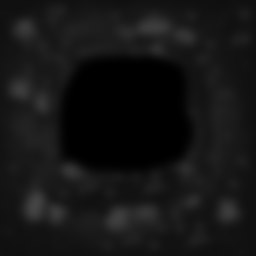
\includegraphics[width=0.3\textwidth]{images/terreno.jpg}
    \caption{Imagem Original em terrains/terreno.jpg}
\end{figure}

\begin{figure}[H]
    \centering
    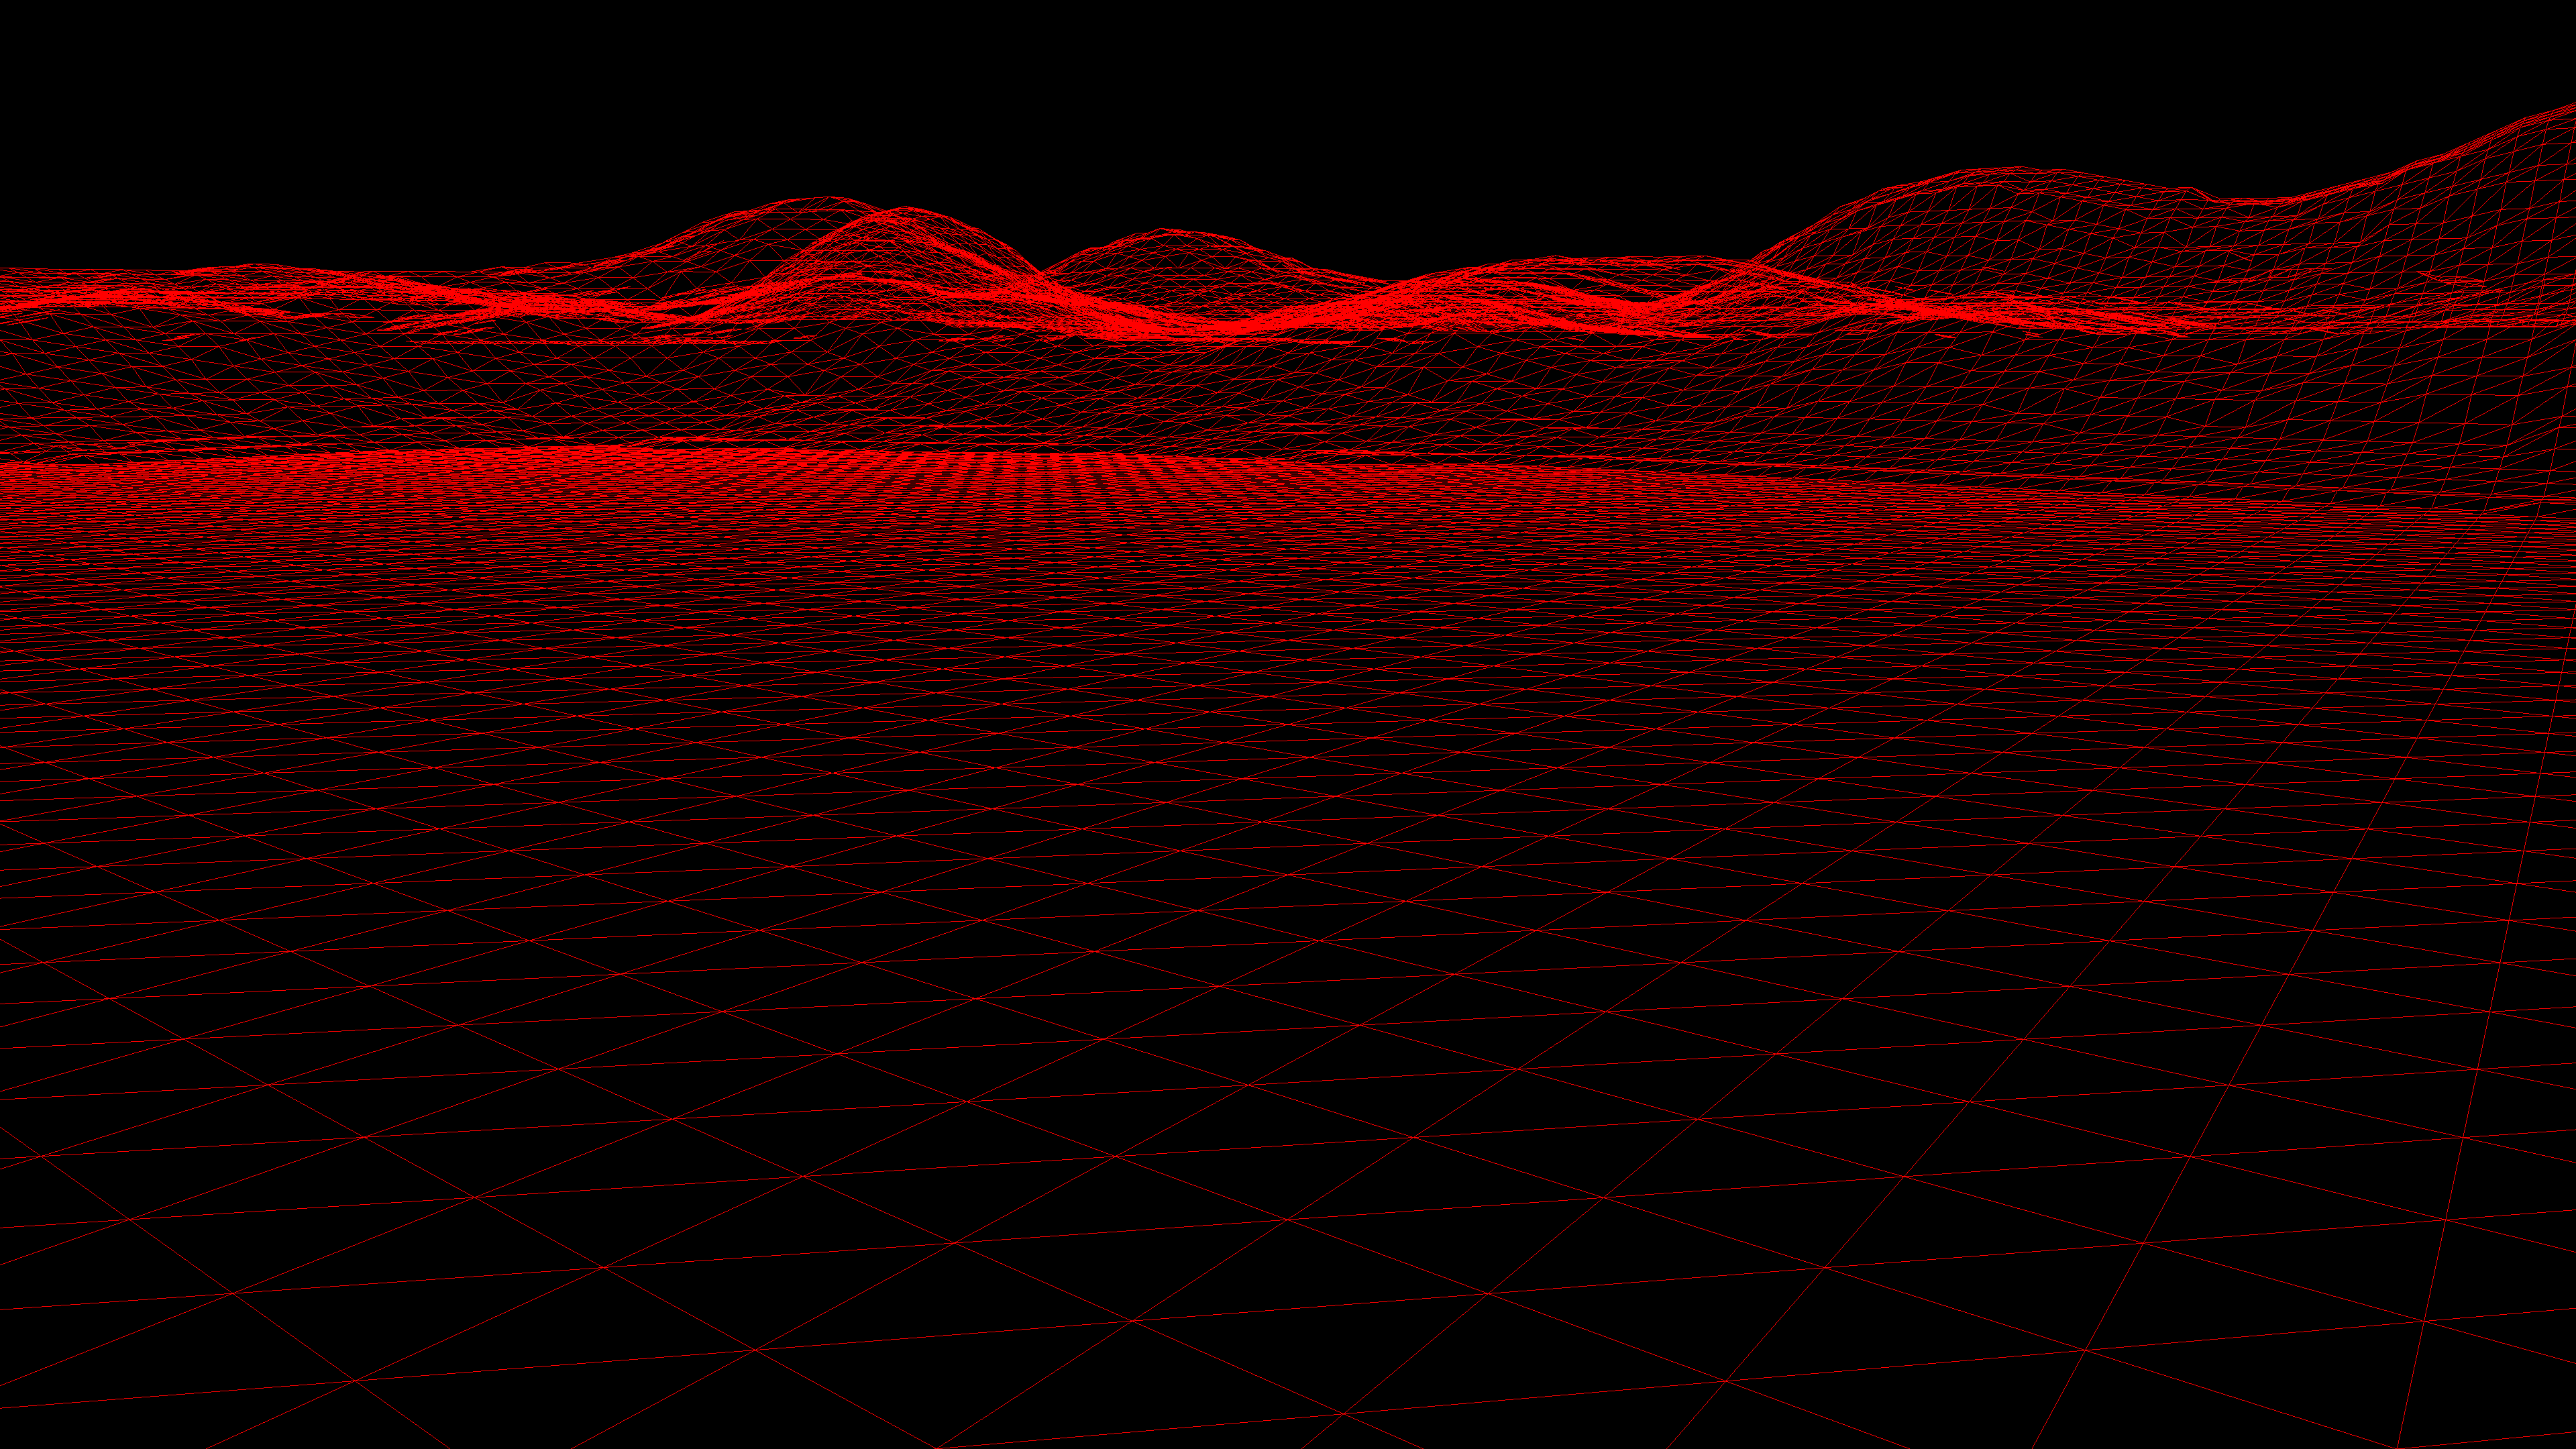
\includegraphics[width=0.5\textwidth]{images/terrain_rendered.png}
    \caption{Resultado do XML}
\end{figure}
Para conseguir carregar o terreno foi expandido sobre o que tinha sido
desenvolvido anteriormente para carregar um modelo.\\
À semelhança de um \textit{ModelBuffer} desenvolvemos um \textit{TerrainBuffer}.
Este último contem um buffer, e as dimensões da imagem carregada em pixeis.\\
Assim, quando se quer carregar uma imagem para um VBO basta usar o construtor
desta classe, sendo que o fileName é o caminho para a imagem e o
\textit{min\_height} e \textit{max\_height} é o novo intervalo em que se
encontram os valores de altura.\\
Primeiro a imagem é carregada usando \textit{DevIL} para memória
(\textit{imageData}).\\
Depois são construídos os pontos num vetor. 

\begin{lstlisting}
// 	Build the vertex arrays
std::vector<float> vec;
i32 new_interval = max_height - min_height;
for (i32 h = 0; h < _image_height; h++) {
    for (i32 w = 0; w < _image_width; w++) {
        float point = imageData[_image_height * h + w];
        float n_point = imageData[_image_height * (h + 1) + w];

        vec.push_back(w - (_image_width / 2.0));                     // x1
        vec.push_back(point * new_interval / 255.0f + min_height);   // y1
        vec.push_back(h - (_image_height / 2.0));                    // z1
        vec.push_back(w - (_image_width / 2.0));                     // x2
        vec.push_back(n_point * new_interval / 255.0f + min_height); // y2
        vec.push_back(h + 1.0 - (_image_height / 2.0));              // z2
    }
}
\end{lstlisting}

Por fim o buffer é inicializado e o vetor é copiados para o buffer.\\
Seguindo a mesma lógica, acrescentamos ao \textit{GroupBuffer} outro
\textit{unordered\_map} que associa o nome da imagem a um \textit{TerrainBuffer}
correspondente e criamos o método \textit{draw\_terrain} que procura nesse
\textit{unordered\_map} e desenha.\\
Depois acrescentamos à estrutura recursiva que reflete o XML (\textit{Group}) um
vetor de \textit{Objects} que representam os Terrenos carregados nesse nodo.

\section{Keybinds}
\begin{itemize}
    \item \textit{wasd}: mover camera
    \item \textit{hjkl}: orbitar camera
    \item \textit{p}: toggle pausa
    \item \textit{[ ]}: abrandar/acelerar tempo
    \item \textit{g}: toggle debug mode
        \subitem toggle eixos
        \subitem toggle fps counter (no nome da janela)
        \subitem toggle mostrar TIME\_SCALE (no nome da janela)
        \subitem toggle caminhos de transformação
\end{itemize}
Para implementar a pausa calculamos o tempo entre cada frame. Assim, só se
incrementa um \textit{static u64 elapsed} caso não se esteja em pausa.\\
Para suportar acelerar e abrandar o tempo basta definir um \textit{TIME\_SCALE}
e incrementar e decrementar com base na tecla premida. Depois quando se
incrementa o \textit{elapsed} basta multiplicar o delta pelo
\textit{TIME\_SCALE}.\\

\begin{lstlisting}
//calculate current elapsed
static u64 elapsed = 0;
auto delta = frame_delta();
if (!PAUSE)
    elapsed += delta * TIME_SCALE;
\end{lstlisting}

\chapter{Generator}
Neste módulo foram definidas nas fases anterior 6 primitivas:
\begin{itemize}
        \item Plano
        \item Caixa
        \item Esfera
        \item Cone
        \item Cilindro
        \item Torus
\end{itemize}
Nesta fase implementamos a capacidade do generator interpretar \textit{Patches
de Bezier}.

\section{Patches de Bezier}
\subsection{Parsing}
Primeiro damos parse ao nível de \textit{tesselation}
(\textit{\_tesselation\_level}).\\
Para ler os dados presentes no ficheiro primeiro lemos o número de patches
presentes (\textit{\_n\_patches}). Em seguida lemos os n patches seguintes e
guardamos num vetor de vetores (\textit{\_index\_patches}). Depois está presente
o número de pontos de controlo (\textit{\_n\_control\_points}). Por fim lemos os
n pontos seguintes para um vetor de pontos (\textit{\_control\_points}).

\subsection{Calcular pontos}
Para calcular os pontos criamos uma função, \textit{bezier\_point}, que calcule
um ponto ao longo de um conjunto de 4 pontos (p0, p1, p2, p3) com base na matriz
de constantes de bezier e o tempo decorrido (t).\\
A parte de calcular as coordenadas do ponto é exatamente igual à parte de
calcular um ponto numa curva de Catmull-Rom tirando a diferença na matriz de
constantes.

\begin{lstlisting}
// bezier matrix
const float m[4][4] = {
    {-1.0f, +3.0f, -3.0f, +1.0f},
    {+3.0f, -6.0f, +3.0f, +0.0f},
    {-3.0f, +3.0f, +0.0f, +0.0f},
    {+1.0f, +0.0f, +0.0f, +0.0f}};
\end{lstlisting}

Em seguida, utilizamos esta função para calcular as coordenadas de um ponto
dentro de um patch. A função criada para isso recebe o índice do patch
(\textit{patch}) e o espaço relativo percorrido para cada lado do patch (u e
v).\\
Primeiro criamos um vetor com todos os pontos que o patch contem. Ou seja,
converter indices de pontos para os pontos em si.\\
Depois aplicamos a função calculada para obter o ponto com as coordenadas u
dentro de cada bezier patch de 4 em 4 pontos.\\
Depois aplicamos novamente essa conta aos 4 pontos calculados e utilizamos a
mesma função mas desta vez com o v.\\

\begin{lstlisting}
std::vector<Point> patch_control_points;
for (auto const& index : _index_patches[patch]) {
    patch_control_points.push_back(_control_points[index]);
}

std::vector<Point> new_patch_points;
for (auto i = patch_control_points.cbegin();
     i != patch_control_points.cend();
     i += 4) {
    new_patch_points.push_back(bezier_point(u, i[0], i[1], i[2], i[3]));
}

return bezier_point(
    v,
    new_patch_points[0],
    new_patch_points[1],
    new_patch_points[2],
    new_patch_points[3]);
\end{lstlisting}

Dividindo 1 pelo \textit{\_tesselation\_level} obtemos o delta de cada ponto
dentro de um patch.\\
Para obter triangulos válidos é necessário saber os 3 pontos que vêm
imediatamente a seguir ao ponto que está a ser calculado. Para isso basta
calcular as combinações de pontos para \textit{ui + 1} e para \textit{vi + 1}.
\begin{lstlisting}
for (i64 p = 0; p < _n_patches; p++) {
    for (i64 ui = 0; ui < _tesselation_level; ui++) {
        const float uf = ui * delta;
        const float next_uf = (ui + 1) * delta;
        for (i64 vi = 0; vi < _tesselation_level; vi++) {
            const float vf = vi * delta;
            const float next_vf = (vi + 1) * delta;

            auto p0 = patch_generator(p, uf, vf);
            auto p1 = patch_generator(p, uf, next_vf);
            auto p2 = patch_generator(p, next_uf, vf);
            auto p3 = patch_generator(p, next_uf, next_vf);

            coords.push_back(p3);
            coords.push_back(p2);
            coords.push_back(p1);

            coords.push_back(p2);
            coords.push_back(p0);
            coords.push_back(p1);
        }
    }
}
\end{lstlisting}


\chapter{Scenes}
\section{Terrain Generation}
Tal como foi referido acima, quando fizemos a conversão do \textit{engine} para
VBOs fizemos de forma a que cada ficheiro contendo um modelo apenas fosse
carregado para memoria uma vez mesmo que este aparecesse no XML varias vezes.\\
Para demonstrar as vantagens deste método criamos um script em python que gera
uma grelha de cubos com tamanho 200 por 200. Visto que também queríamos tornar
esta \textit{Scene} visualmente apelativa decidimos variar a altura dos cubos com
base em \textit{Perlin Noise} fazendo com que o terreno final se aproxime
bastante do aspeto do jogo \textit{Minecraft}.\\
Visto que ainda não temos nem luz nem texturas, para ser possível distinguir
cada caixa individualmente, o script atribui uma cor aleatória a cada um dos
blocos.\\
O ficheiro gerado em XML encontra-se em \textit{scenes/minecraft.xml}.

\begin{figure}[H]
    \centering 
    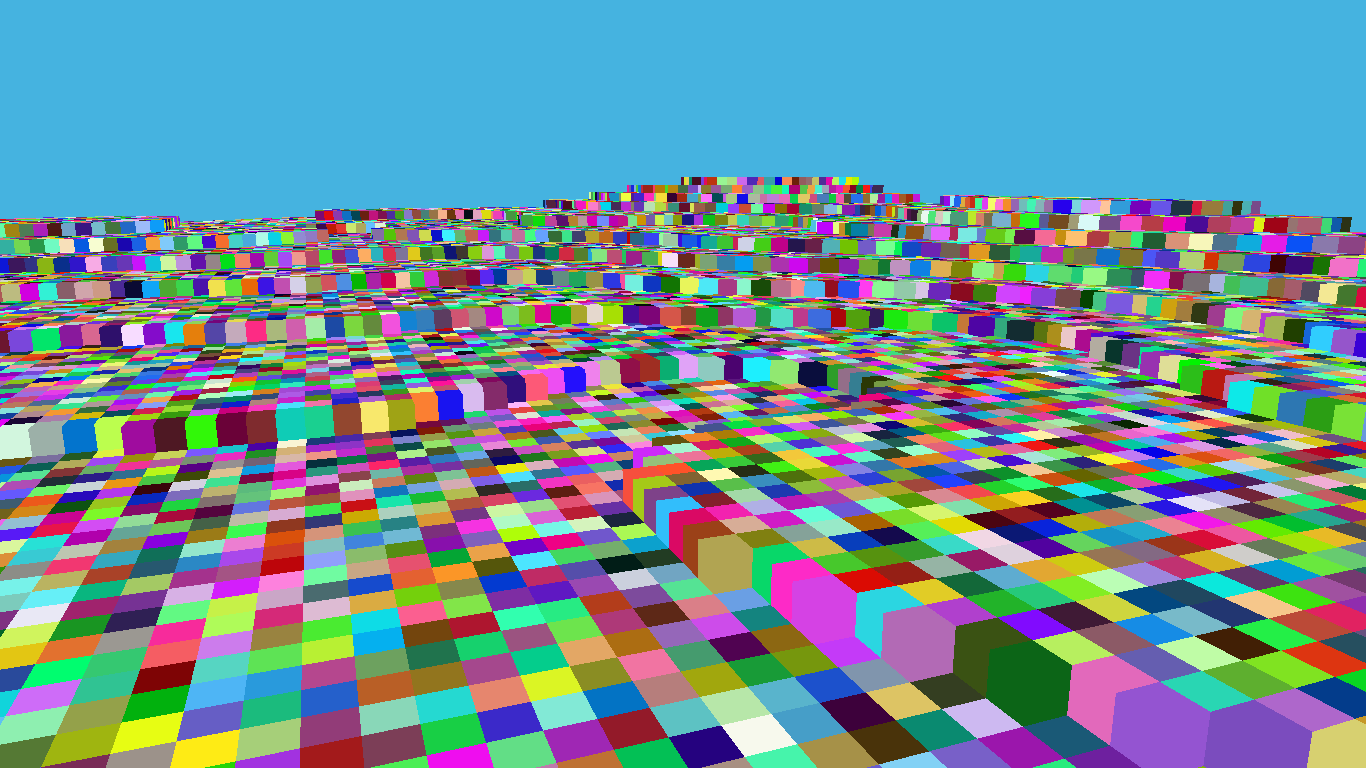
\includegraphics[width=0.8\textwidth]{images/minecraft.png}  
    \caption{Imagem criada}
\end{figure}

\section{Castle in the lake}
Para demonstrar a capacidade das cores terem um fator de transparência e de
carregar imagens como terreno diretamente no XML criamos uma \textit{Scene}
nova. Nesta desenhamos um castelo numa ilha no centro de um lago. O Terreno onde
se assenta o castelo é desenhado com base num \textit{HeightMap} e a água é um
plano com transparência.\\
Como ainda não temos luz nem texturas decidimos colocar vários ângulos para
facilitar a percepção da \textit{Scene} criada.\\
O ficheiro XML encontra-se em \textit{scenes/castle.xml}.

\begin{figure}[H]
    \centering 
    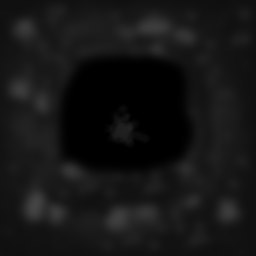
\includegraphics[width=0.4\textwidth]{images/terreno2.jpg}  
    \caption{HeightMap}
\end{figure}

\begin{figure}[H]
    \centering 
    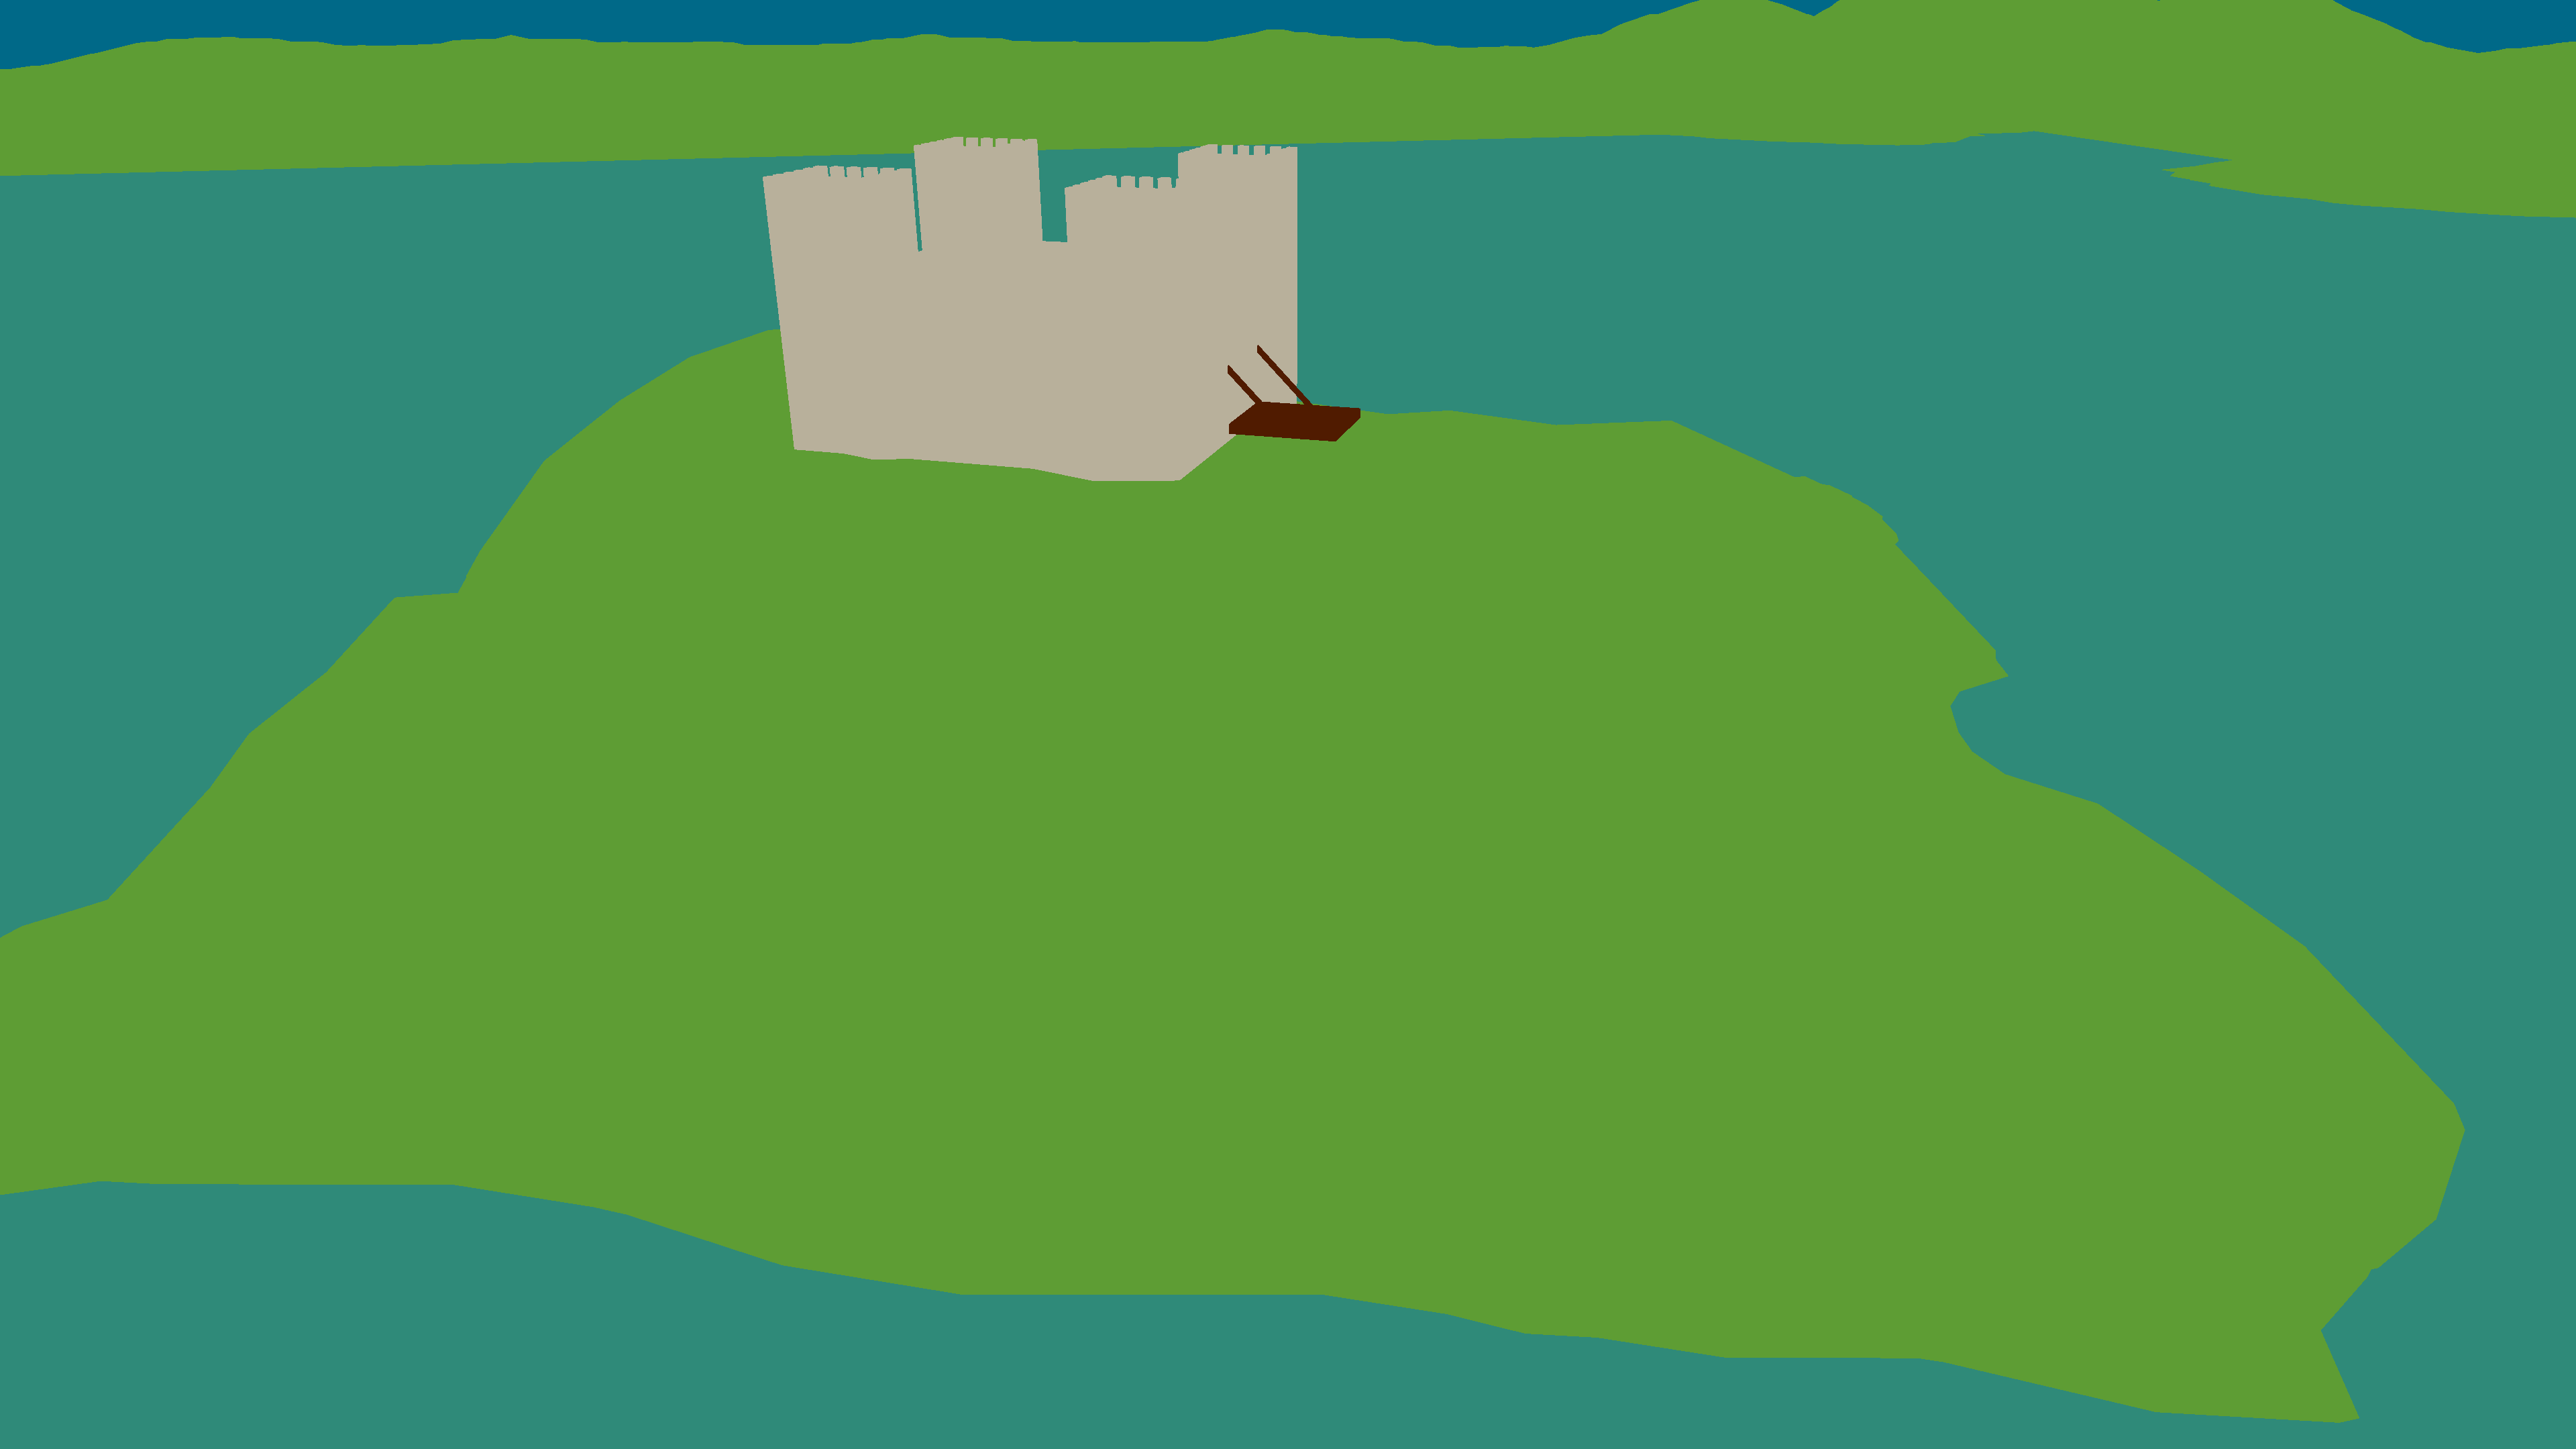
\includegraphics[width=0.6\textwidth]{images/side_castle.png}  
    \caption{lado direito do castelo}
\end{figure}

\begin{figure}[H]
    \centering 
    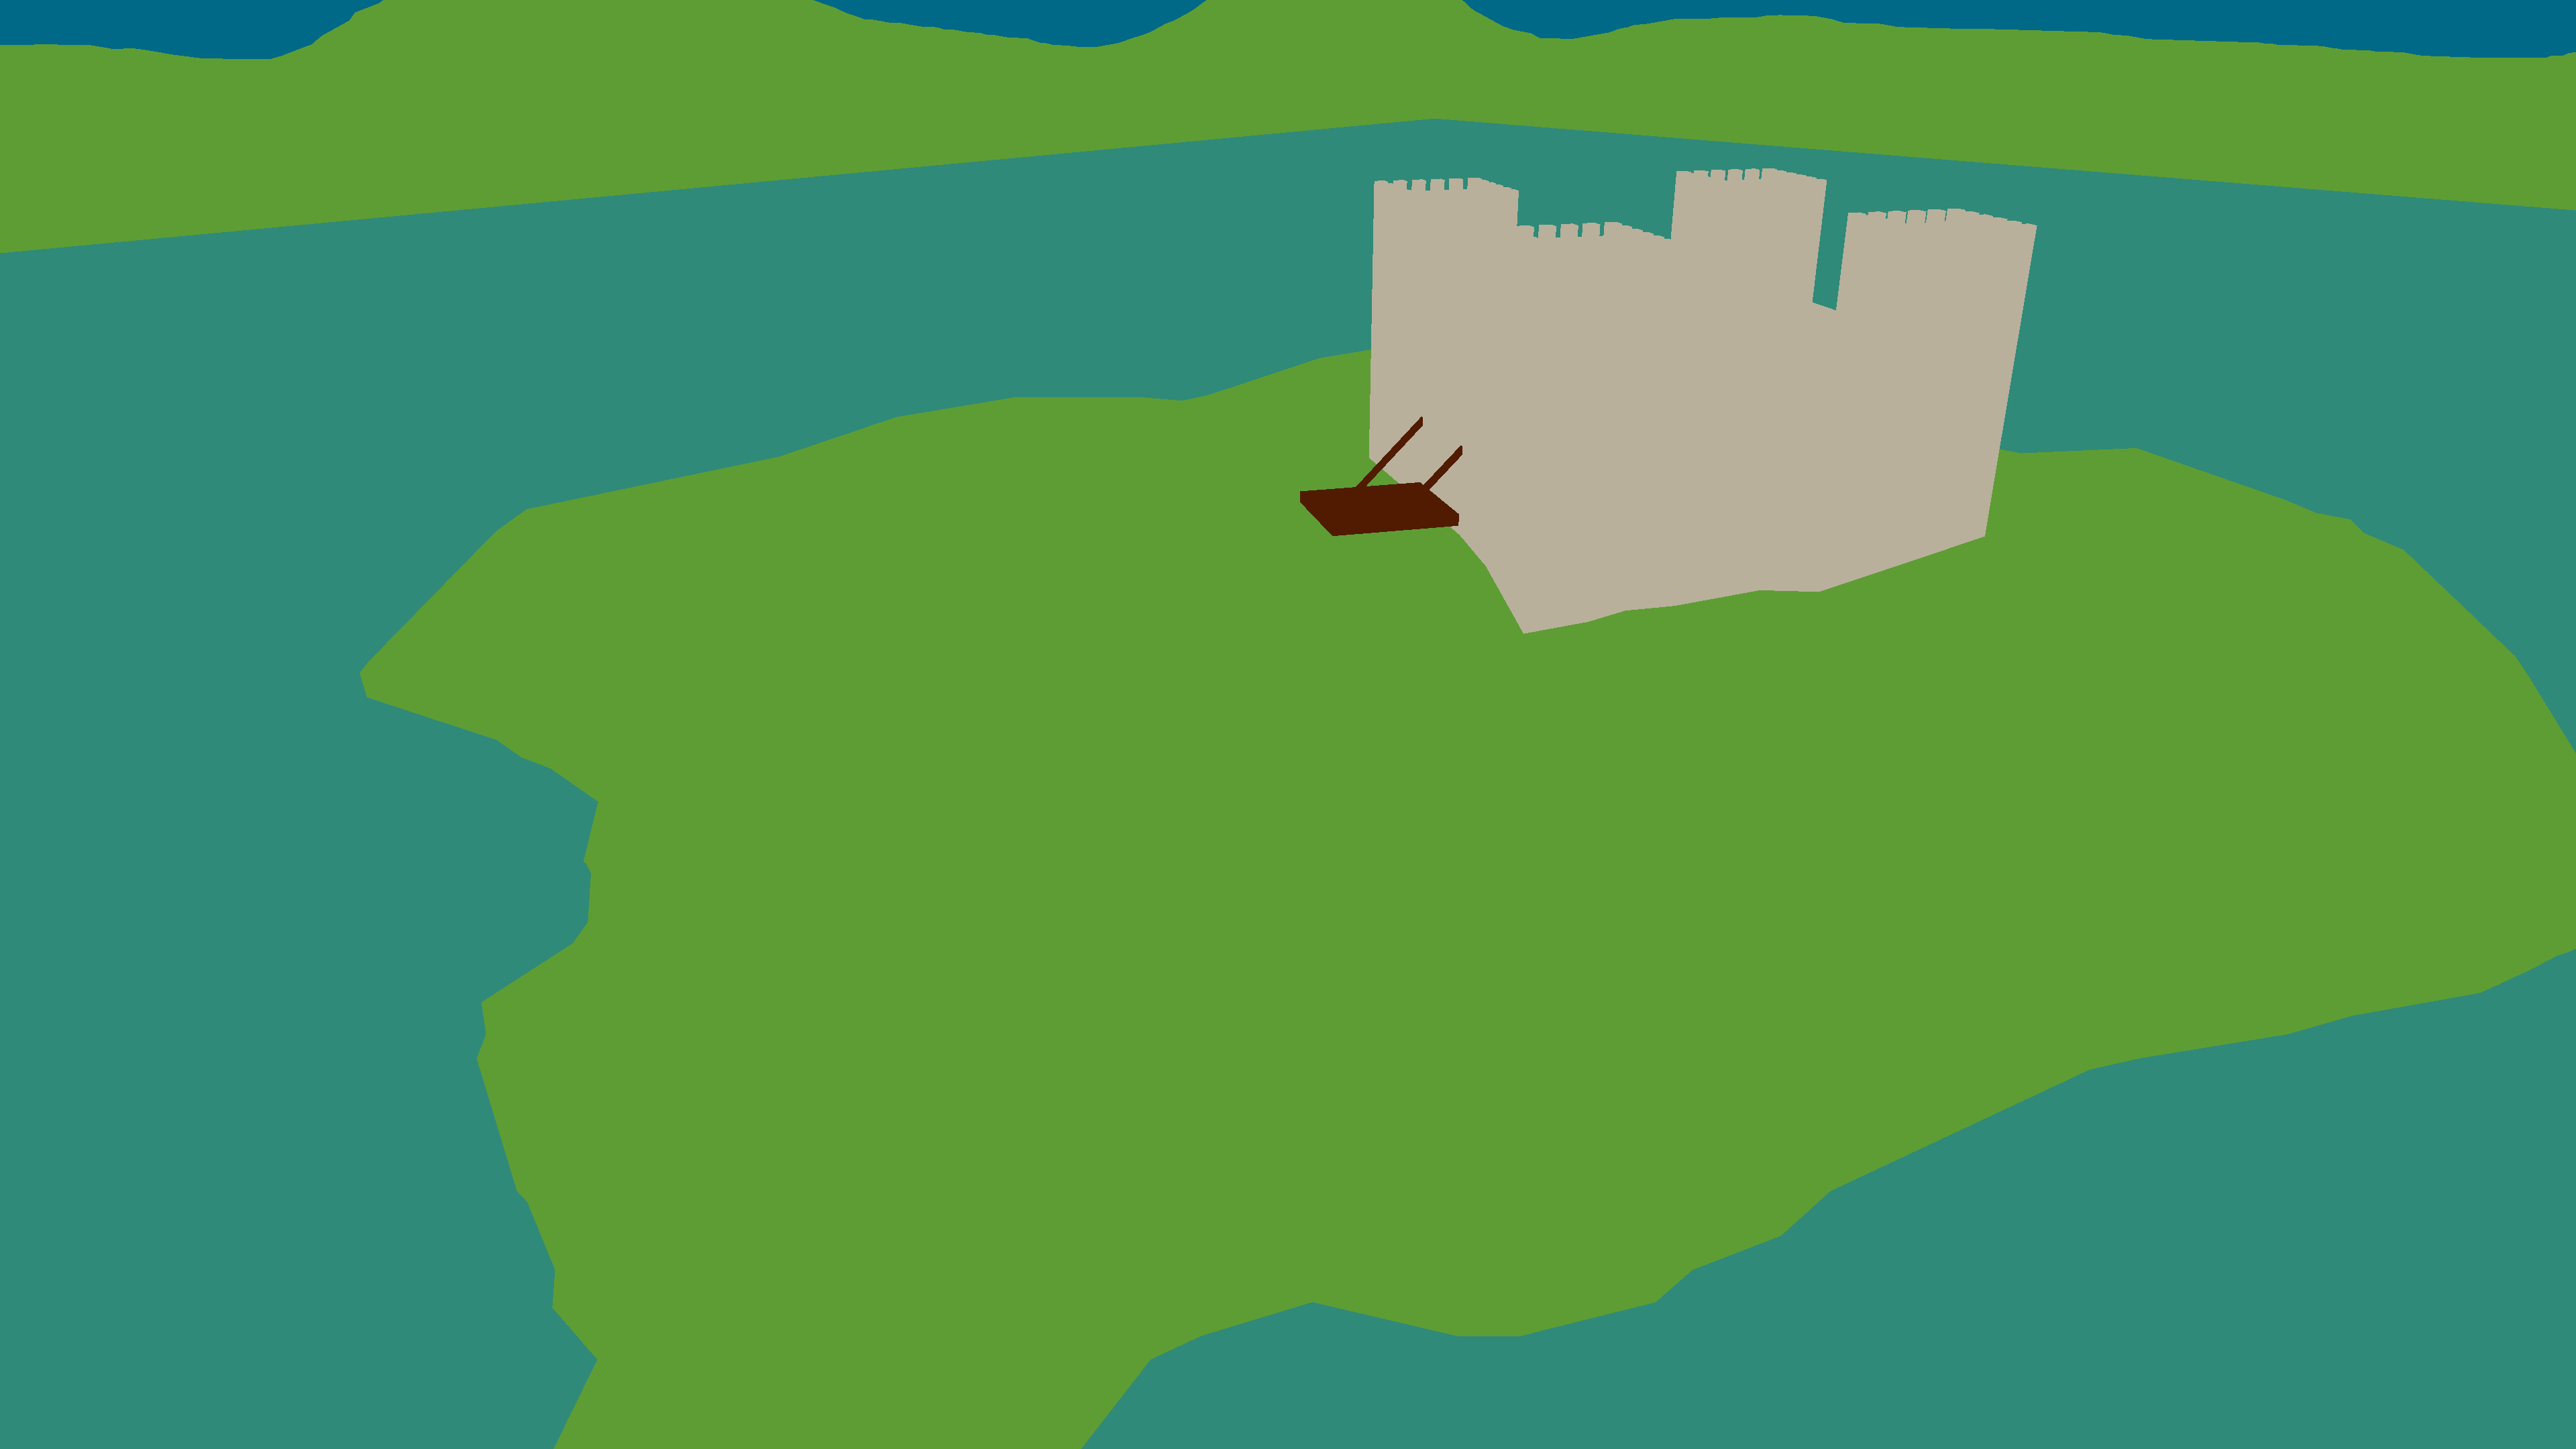
\includegraphics[width=0.6\textwidth]{images/side2_castle.png}  
    \caption{lado esquerdo do castelo}
\end{figure}

\begin{figure}[H]
    \centering 
    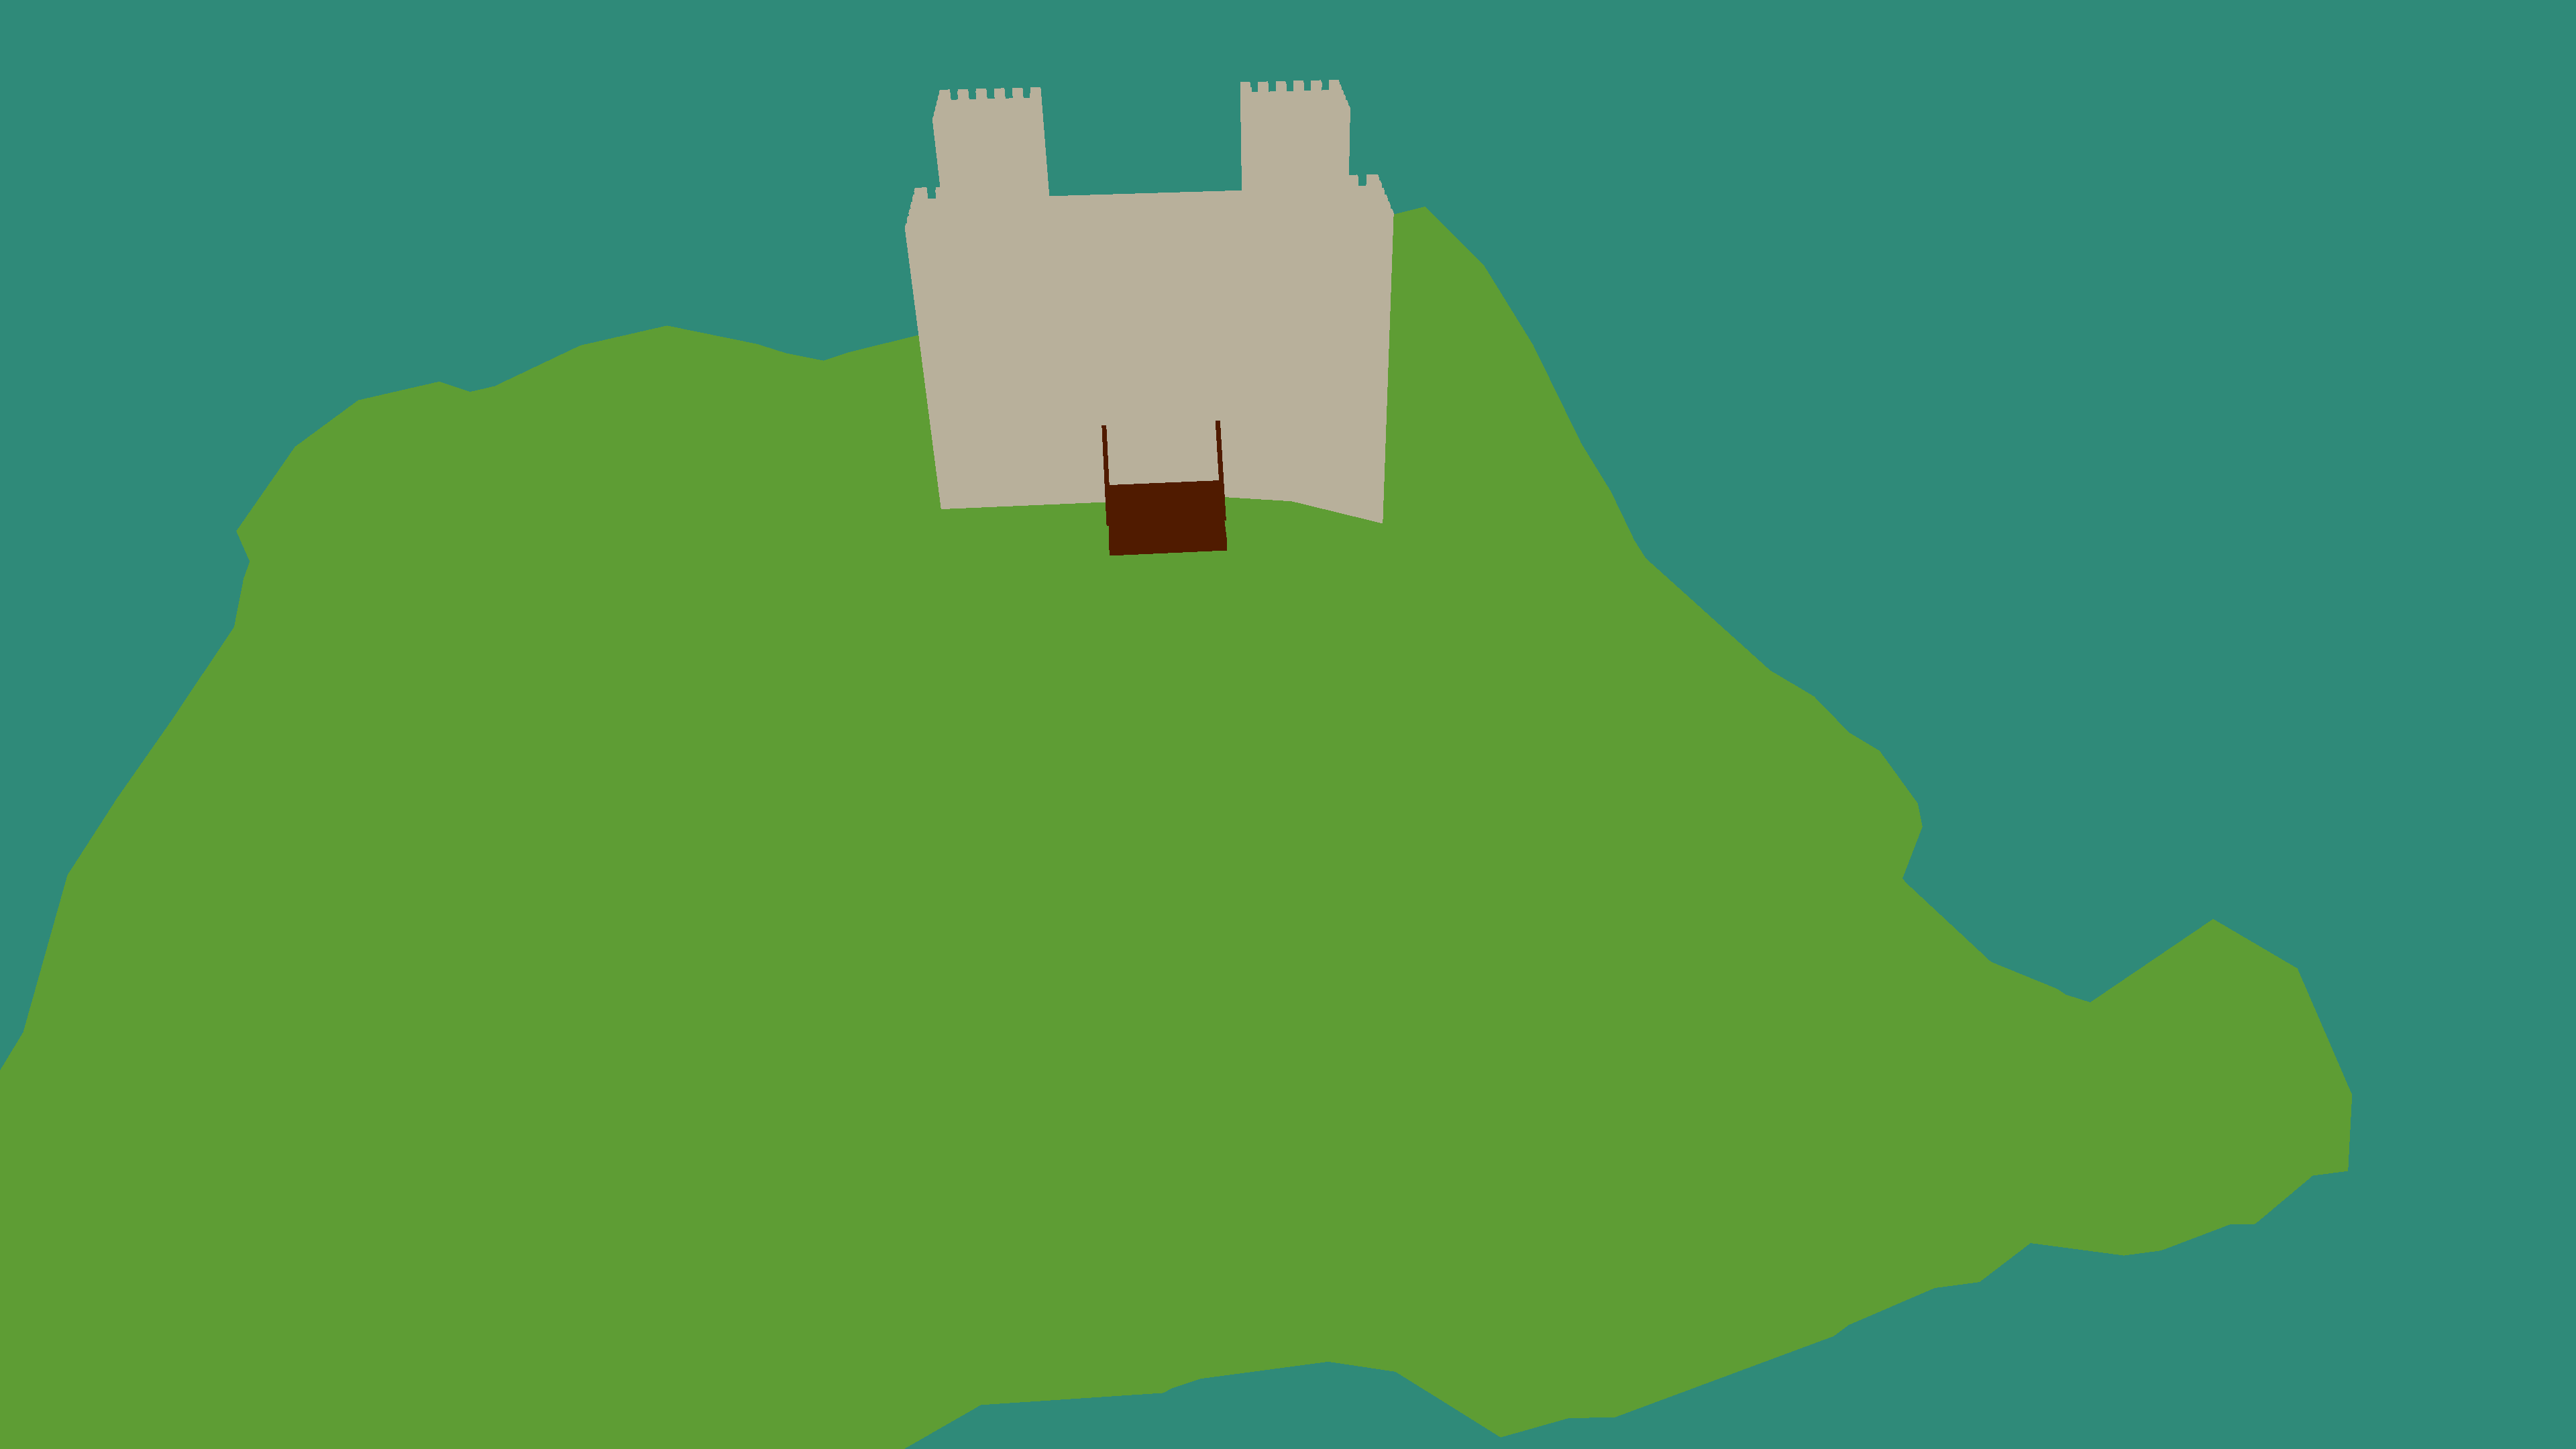
\includegraphics[width=0.6\textwidth]{images/front_castle.png}  
    \caption{lado esquerdo do castelo}
\end{figure}

\section{Solar System}
Para facilitar desenhar o sistema solar decidimos criar um script em Python.\\
De forma a criar um modelo relativamente realista do sistema solar decidimos
seguir um conjunto de regras simples, criando várias escalas permite que seja
criado um modelo relativamente realista do sistema solar mas ao mesmo tempo
visualmente apelativo.\\

\begin{itemize}
        \item tamanho de planetas e luas está à escala entre planetas e luas
        \item distancia dos planetas e cinturas de asteróides ao sol está à
            escala
        \item o tempo de órbita e o tempo de rotação estão à escala mas
            acelerados por fatores diferentes
\end{itemize}
Os \textit{CSV} obtidos na fase anterior forma expandidos para também incluir
informação sobre o tempo de rotação e o tempo de órbita de cada planeta. Também
acrescentamos Ceres, o maior asteróide na cintura de asteróides.\\
A informação acrescentada foi obtida na página de Wikipédia de cada planeta.\\
Para calcular a orbita do cometa decidimos aproxima-la a uma elipse, visto que
esta é a mais próxima possível que pode ser facilmente computada. A fórmula mais
comum de uma elipse é:
\[ \frac{x^2}{a^2} + \frac{y^2}{b^2} = 1 \]
Assim, para calcular uma fórmula para a elipse de um cometa basta descobrir o a
e o b. Os dados mais comuns que se encontram para a orbita de um cometa são a
eccentricity, o perihelion e o aphelions. Assim podemos calcular os valores
acima com.
\[ a = \frac{aphelion + perihelion}{1 + eccentricity} \]
\[ b = a * \sqrt{1 - eccentricity^2} \]
Agora basta calcular os pontos e mover a posição da elipse calculada centrada na
origem.\\
À medida que o cometa se aproxima mais do sol mais depressa se desloca, e quanto
mais se afasta mais devagar se desloca.\\
Visto que podemos representar a órbita de qualquer asteróide decidimos utilizar
os dados do Halley.\\
O ficheiro gerado em XML encontra-se em \textit{scenes/solar.xml}.

\begin{figure}[H]
    \centering 
    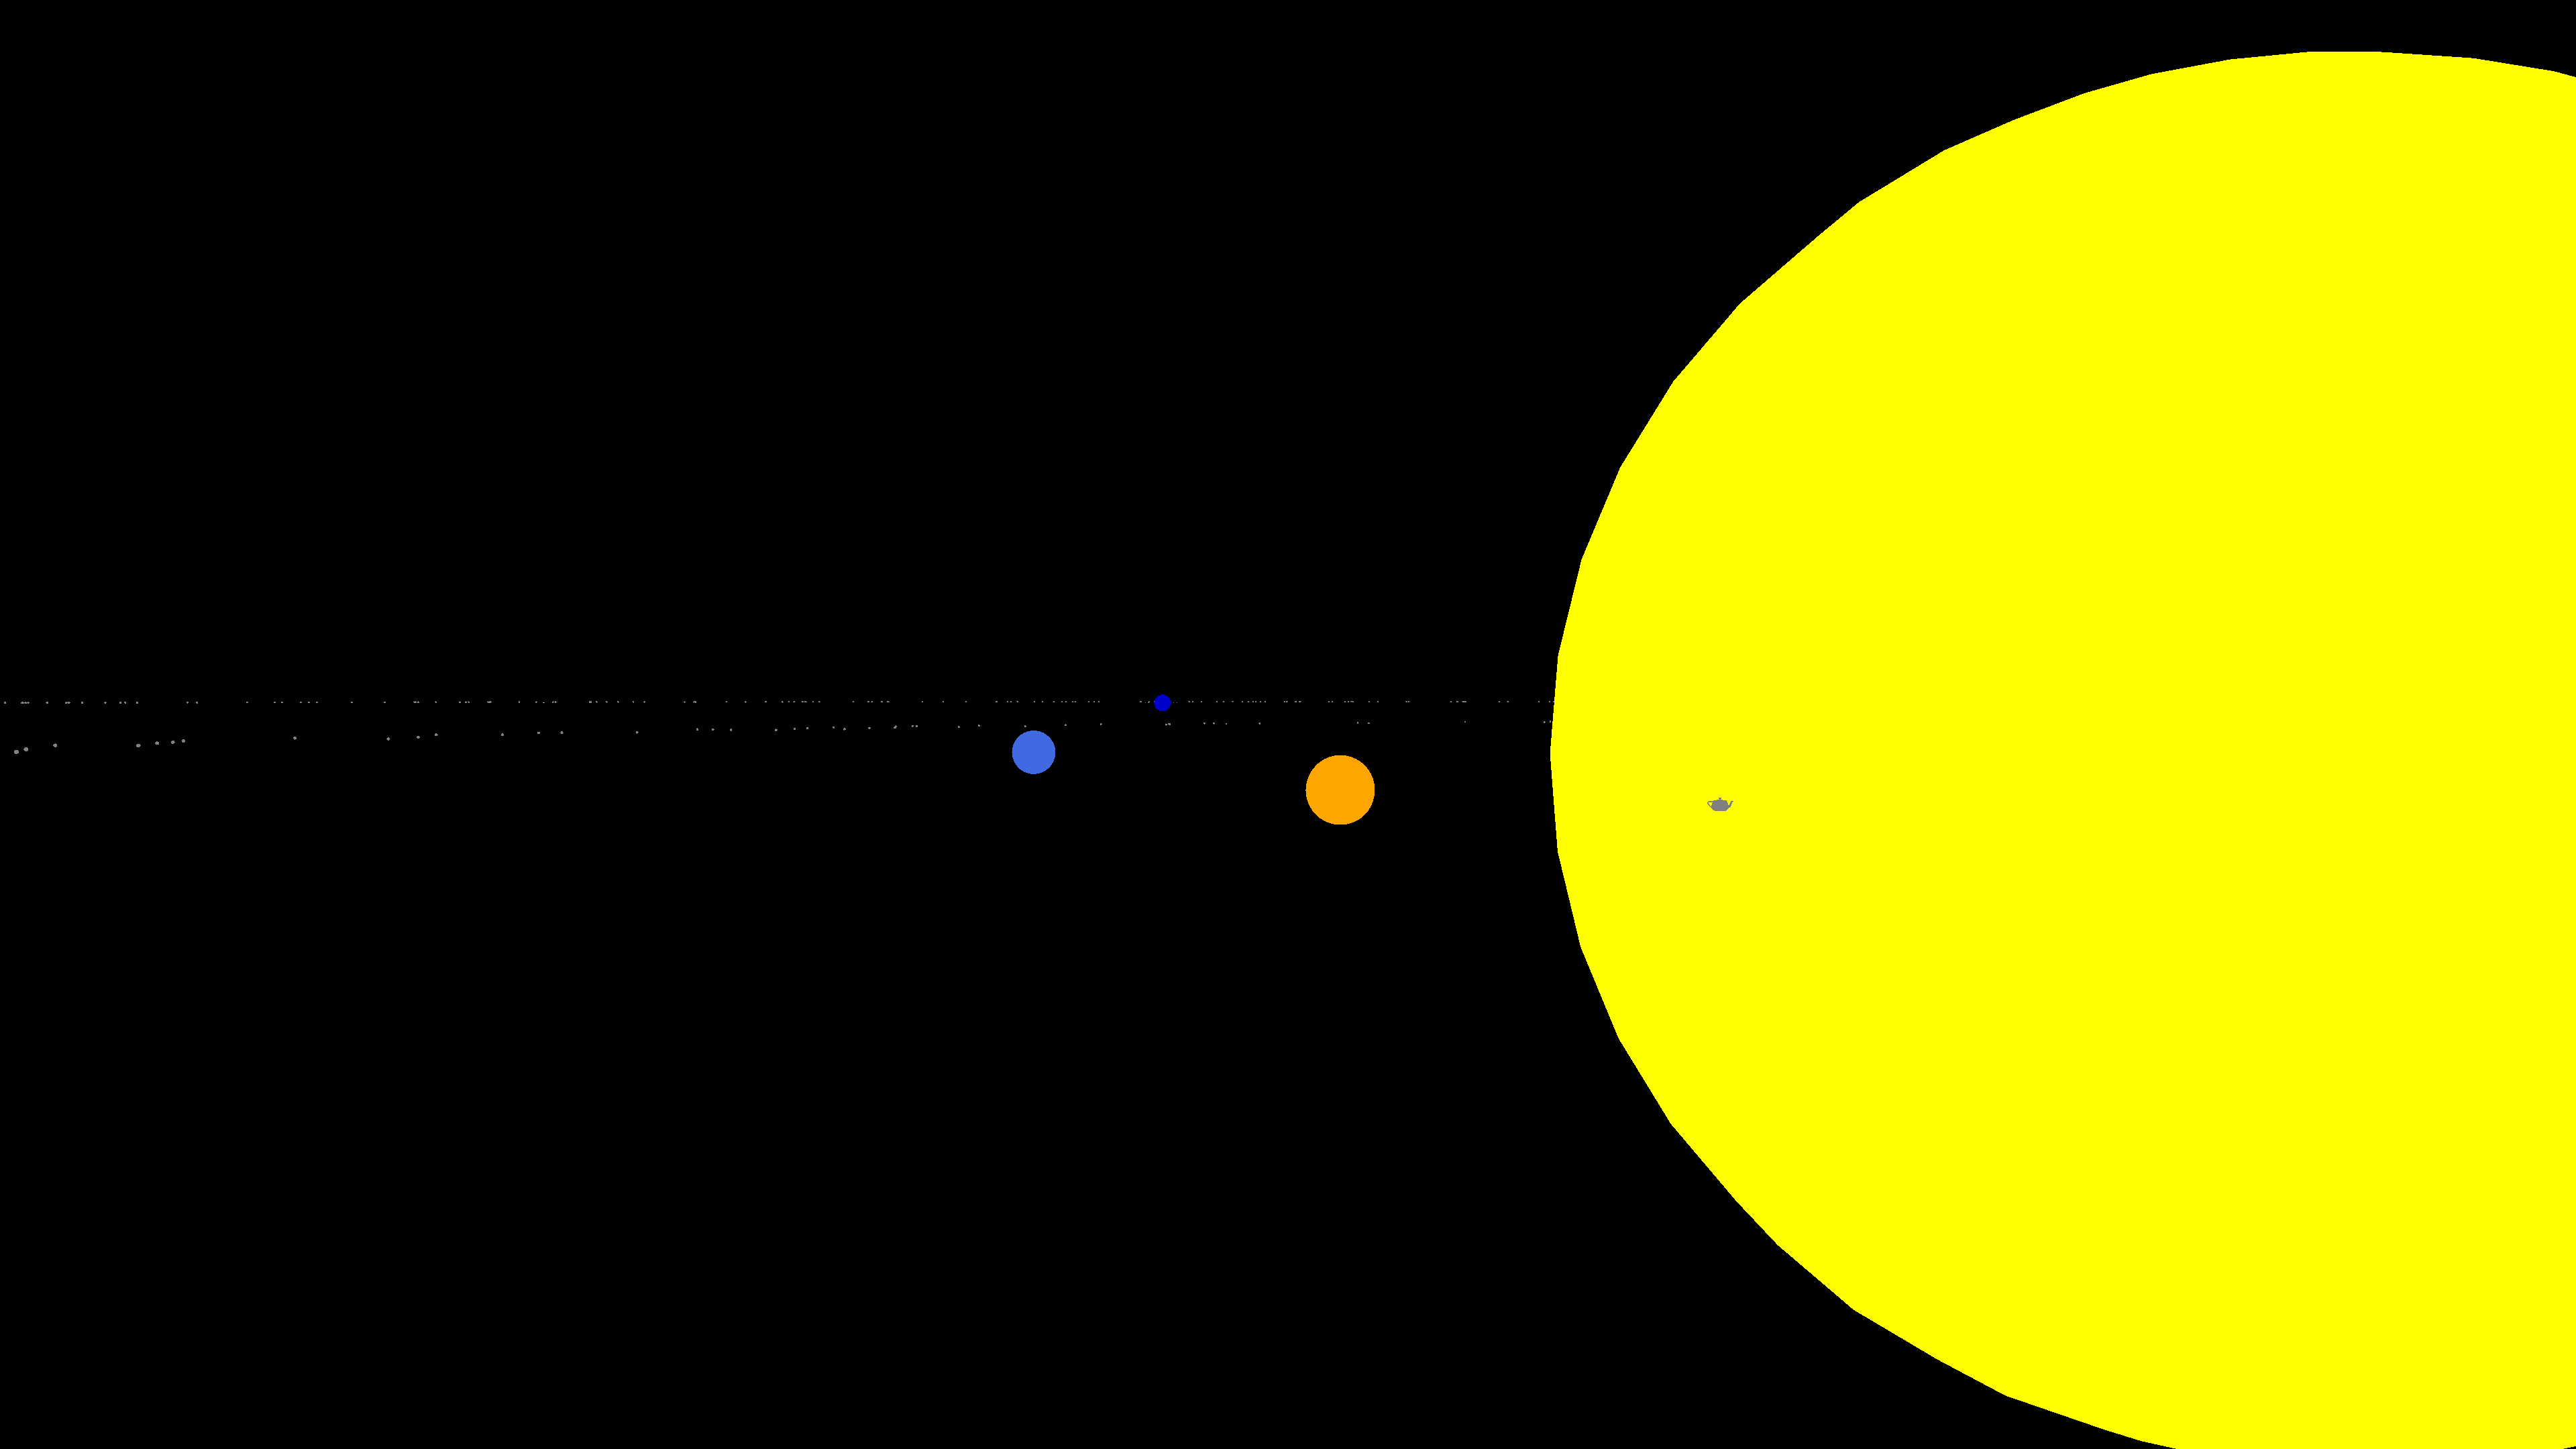
\includegraphics[width=0.7\textwidth]{images/close_view.png}  
    \caption{teapot em frente ao sol}
\end{figure}
\begin{figure}[H]
    \centering 
    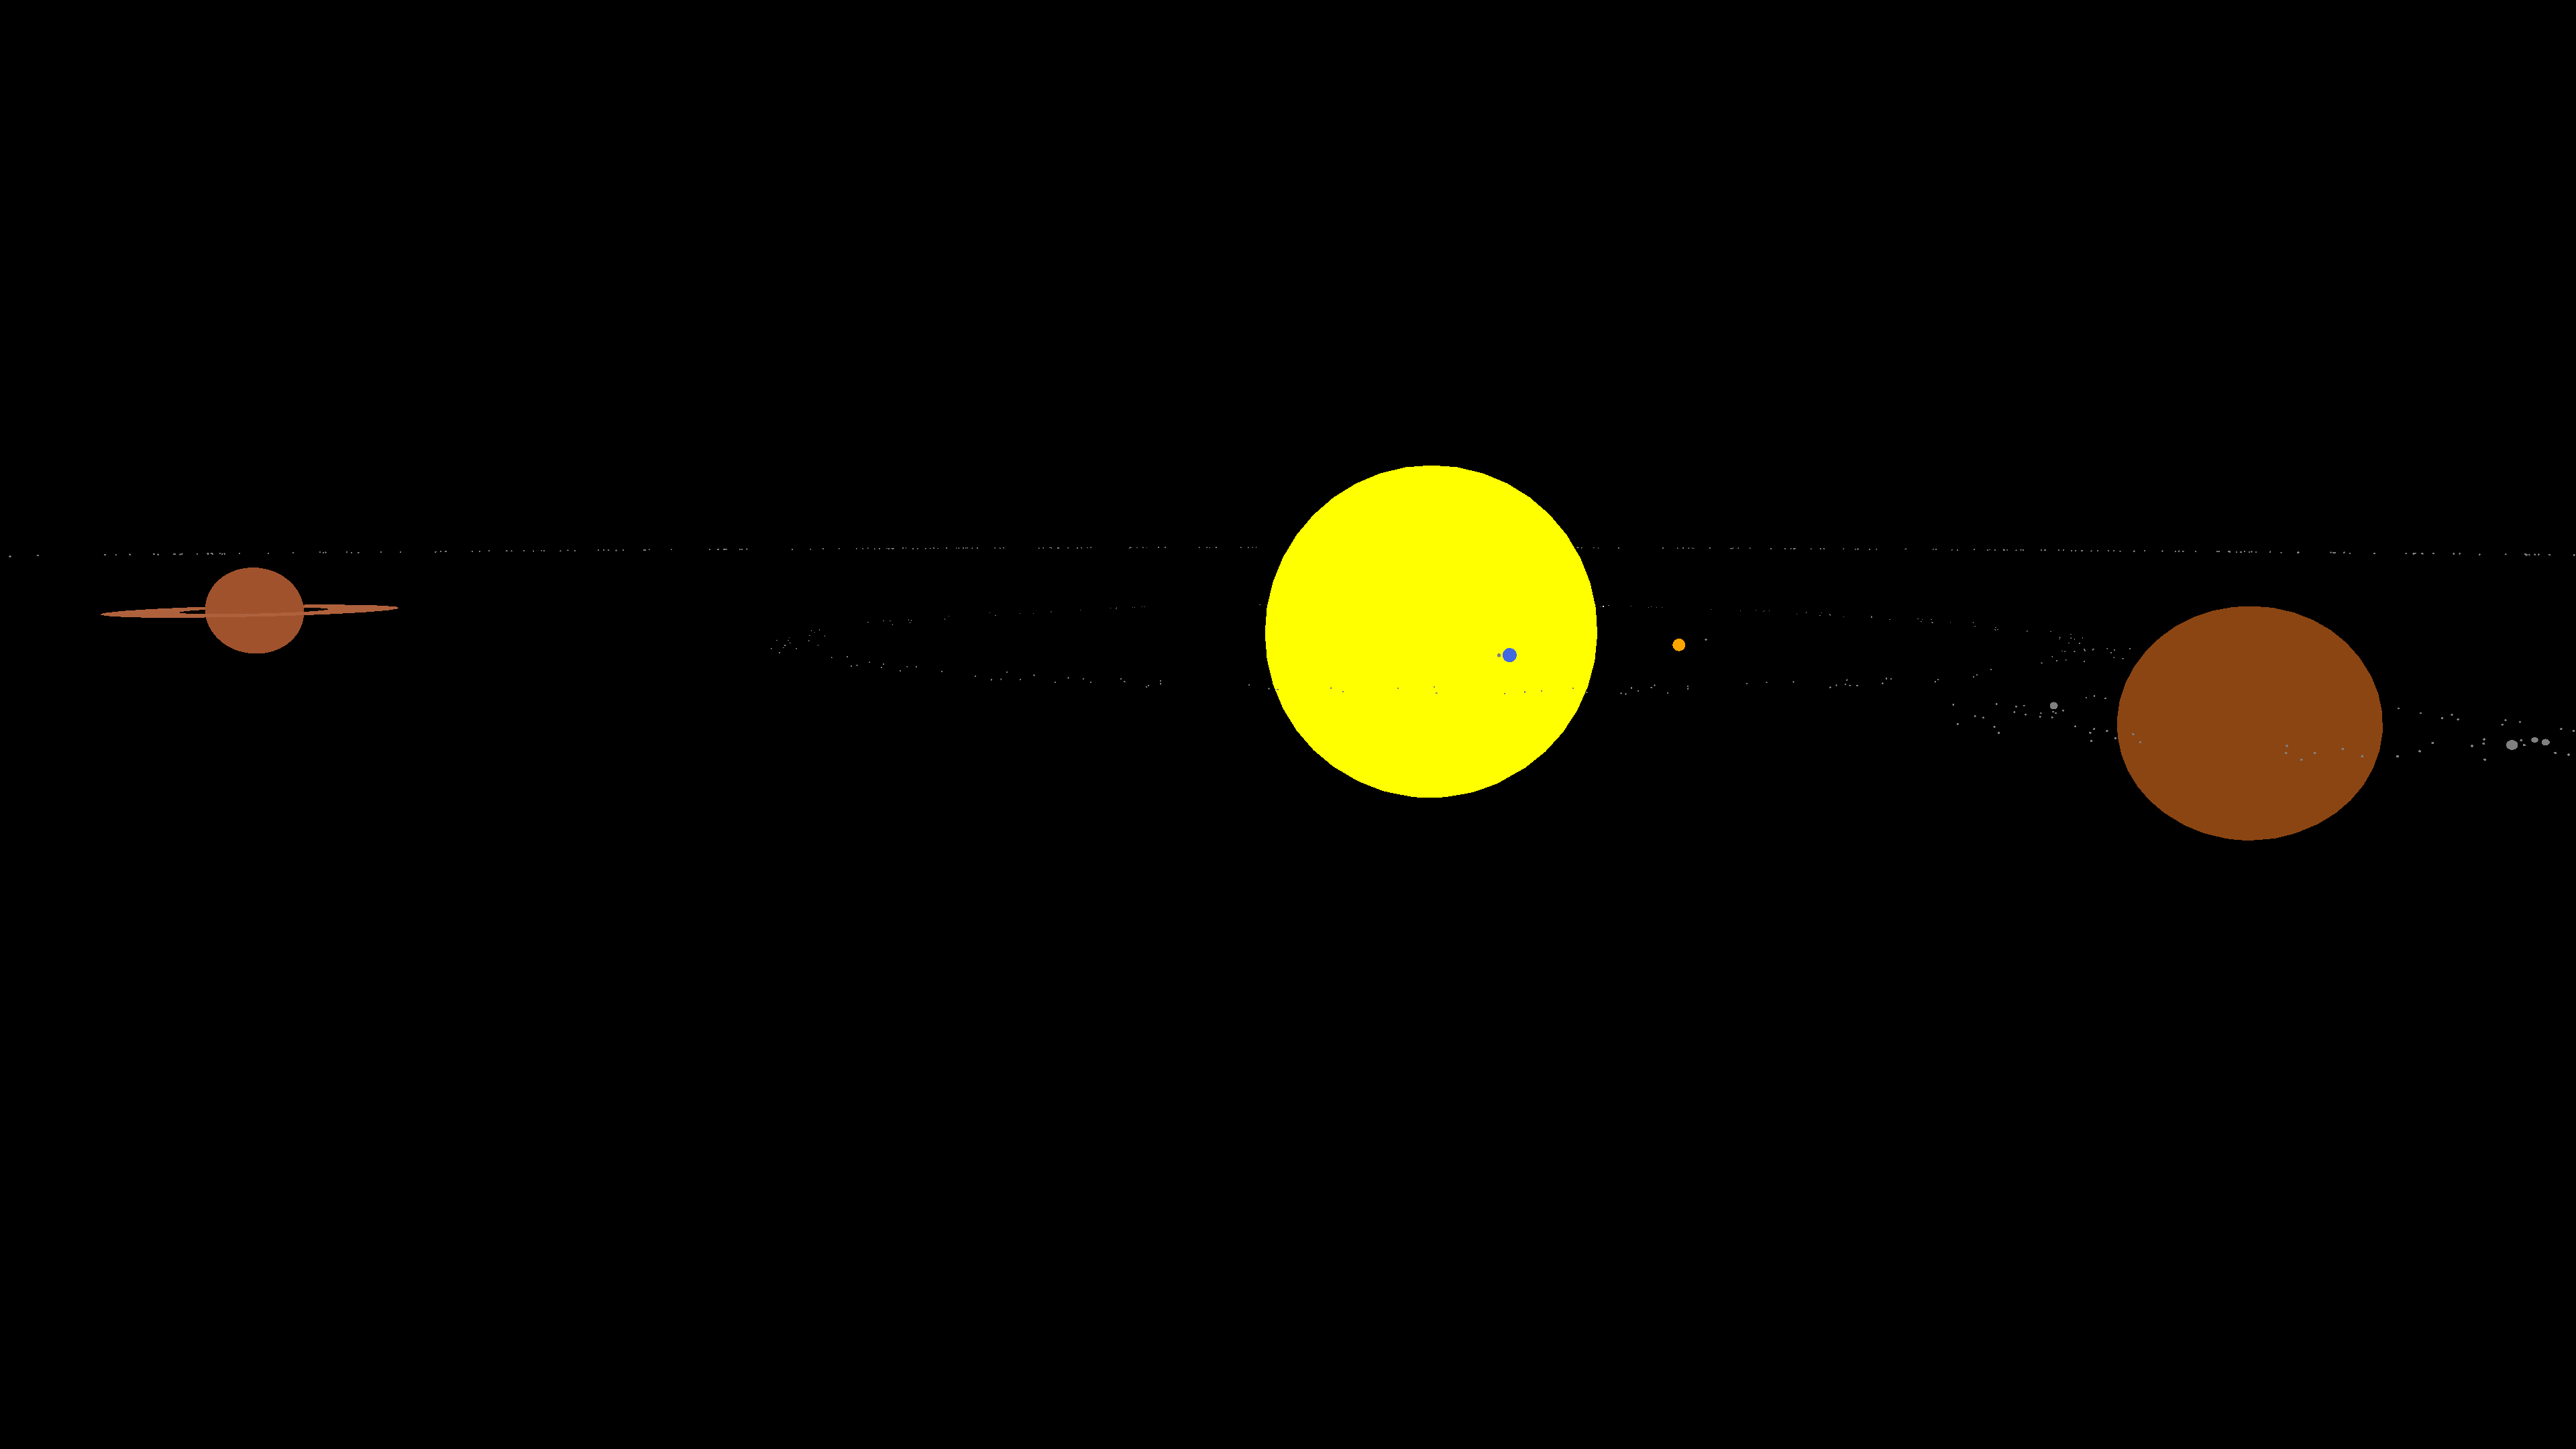
\includegraphics[width=0.7\textwidth]{images/side_view.png}  
    \caption{planetas interiores}
\end{figure}
\begin{figure}[H]
    \centering 
    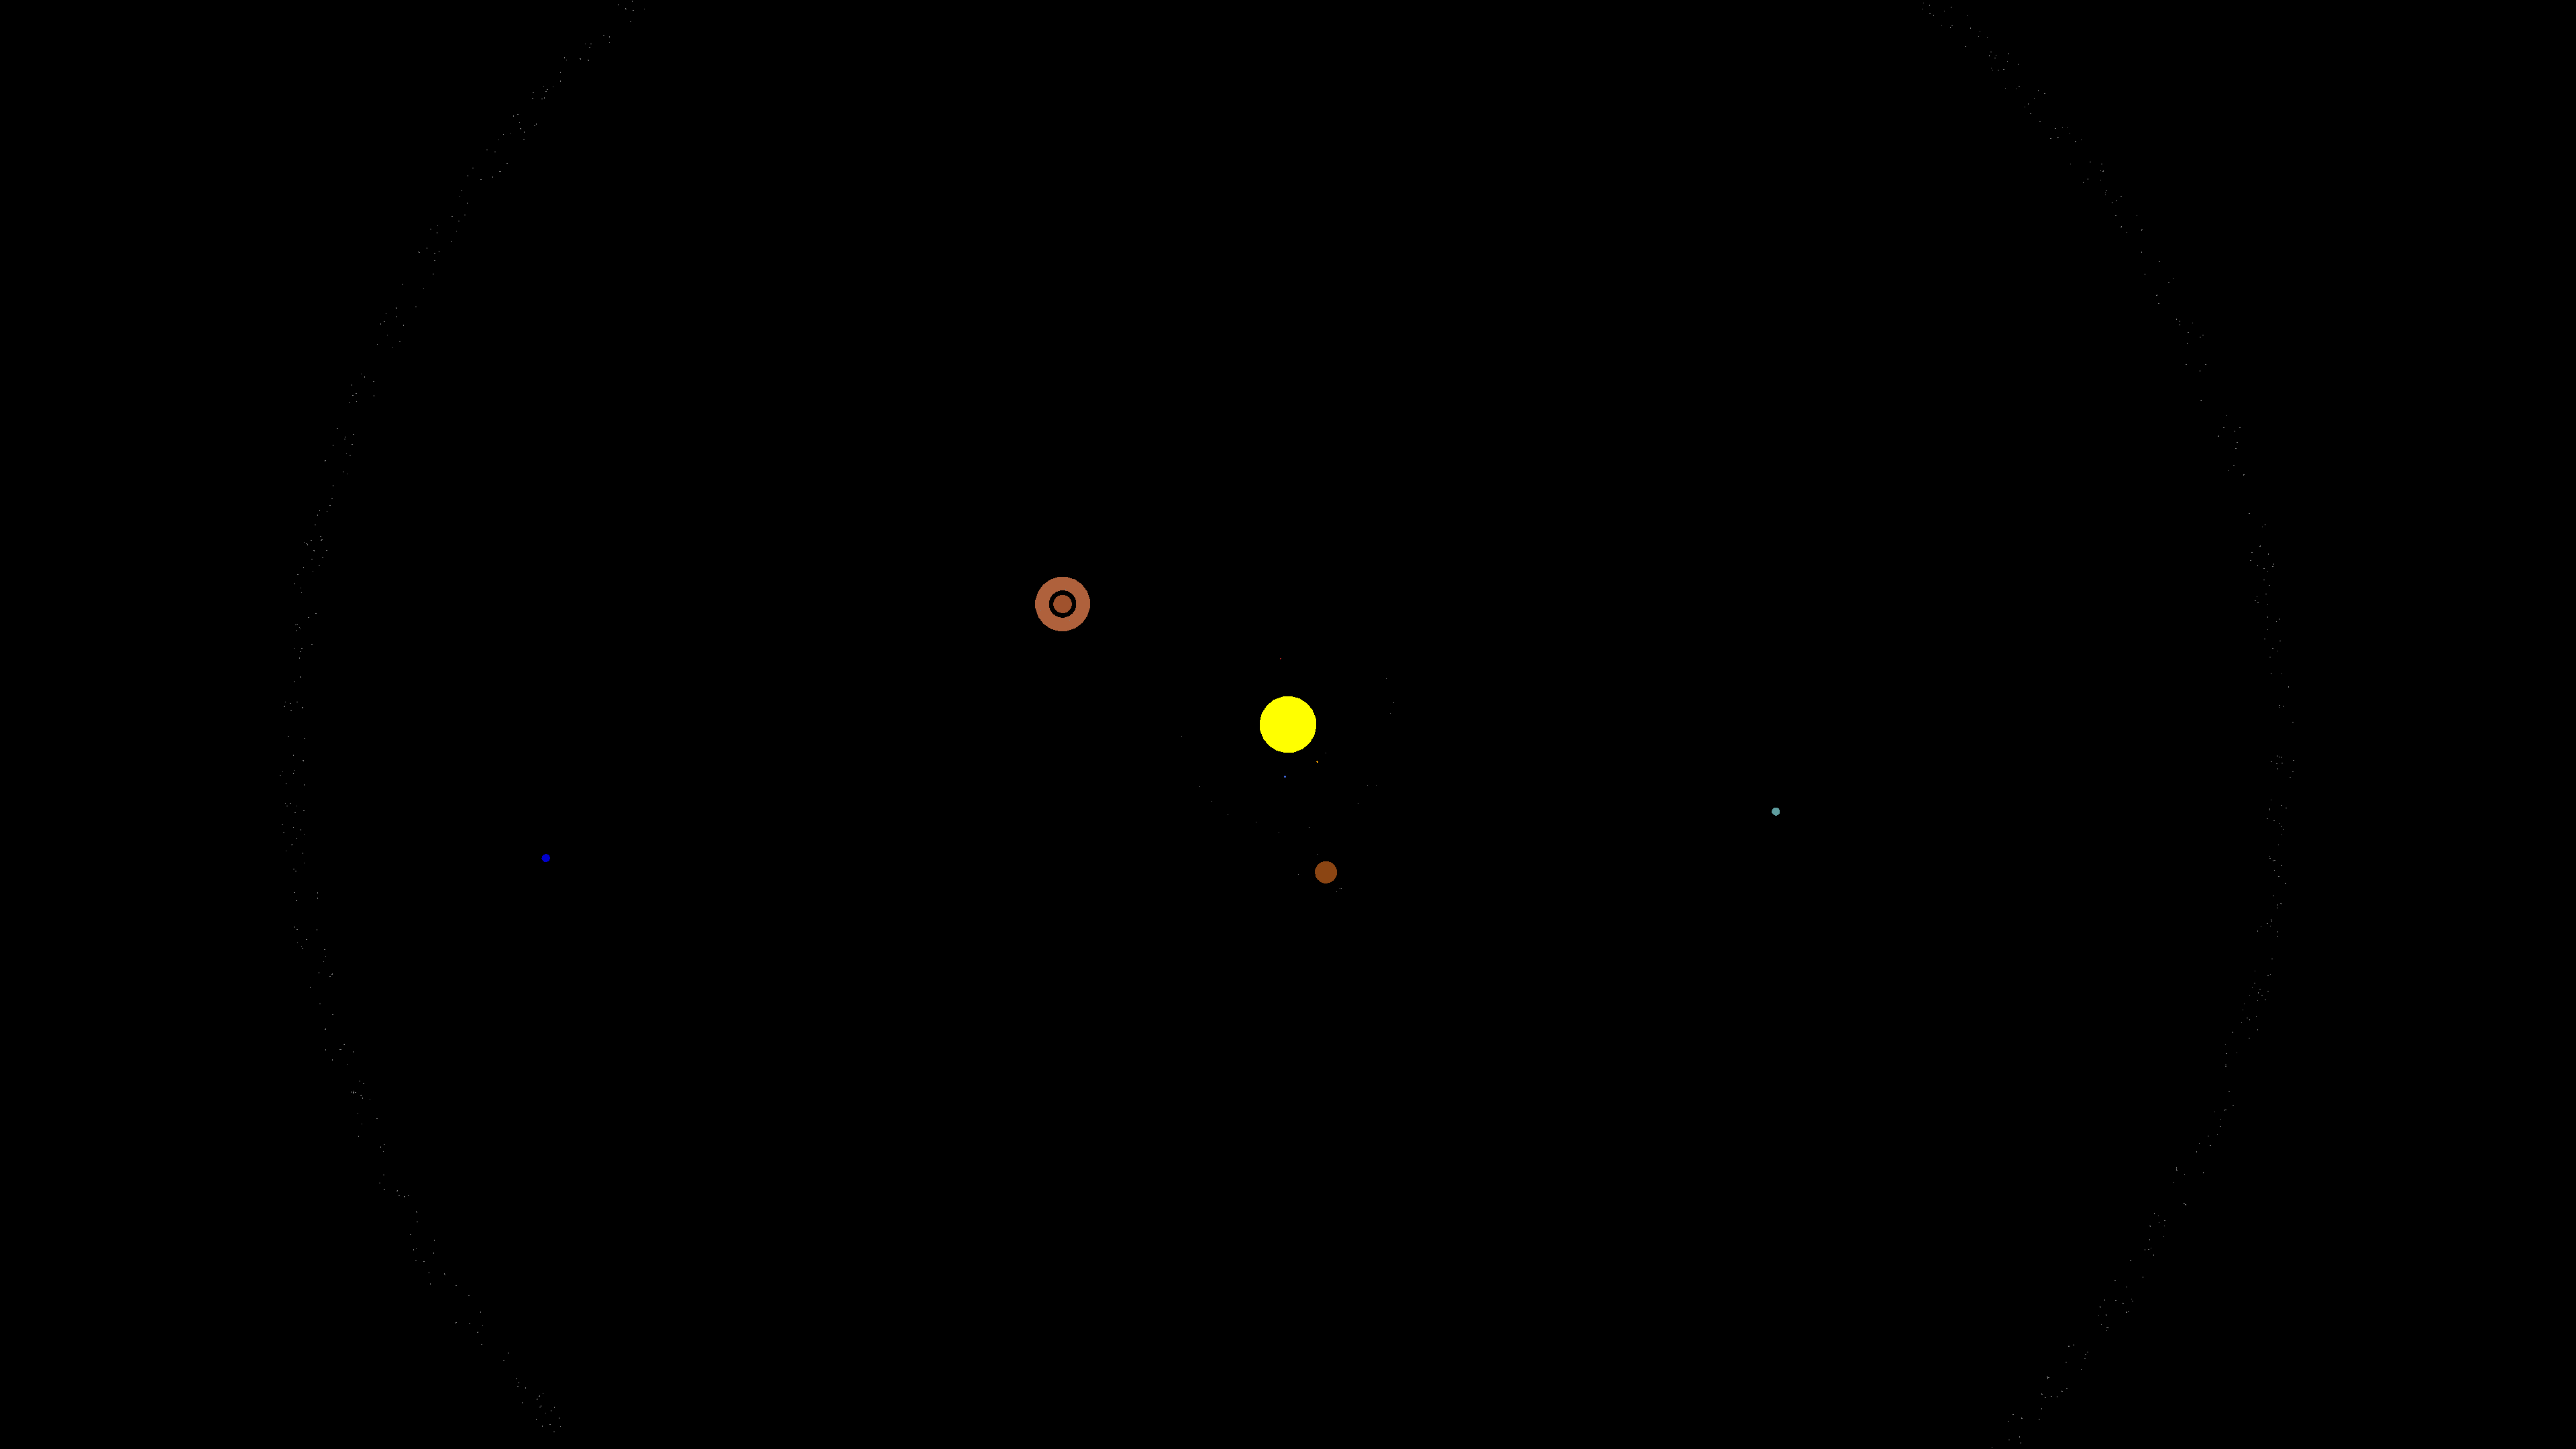
\includegraphics[width=0.7\textwidth]{images/top_view.png}  
    \caption{vista superior do sistema solar}
\end{figure}
\begin{figure}[H]
    \centering 
    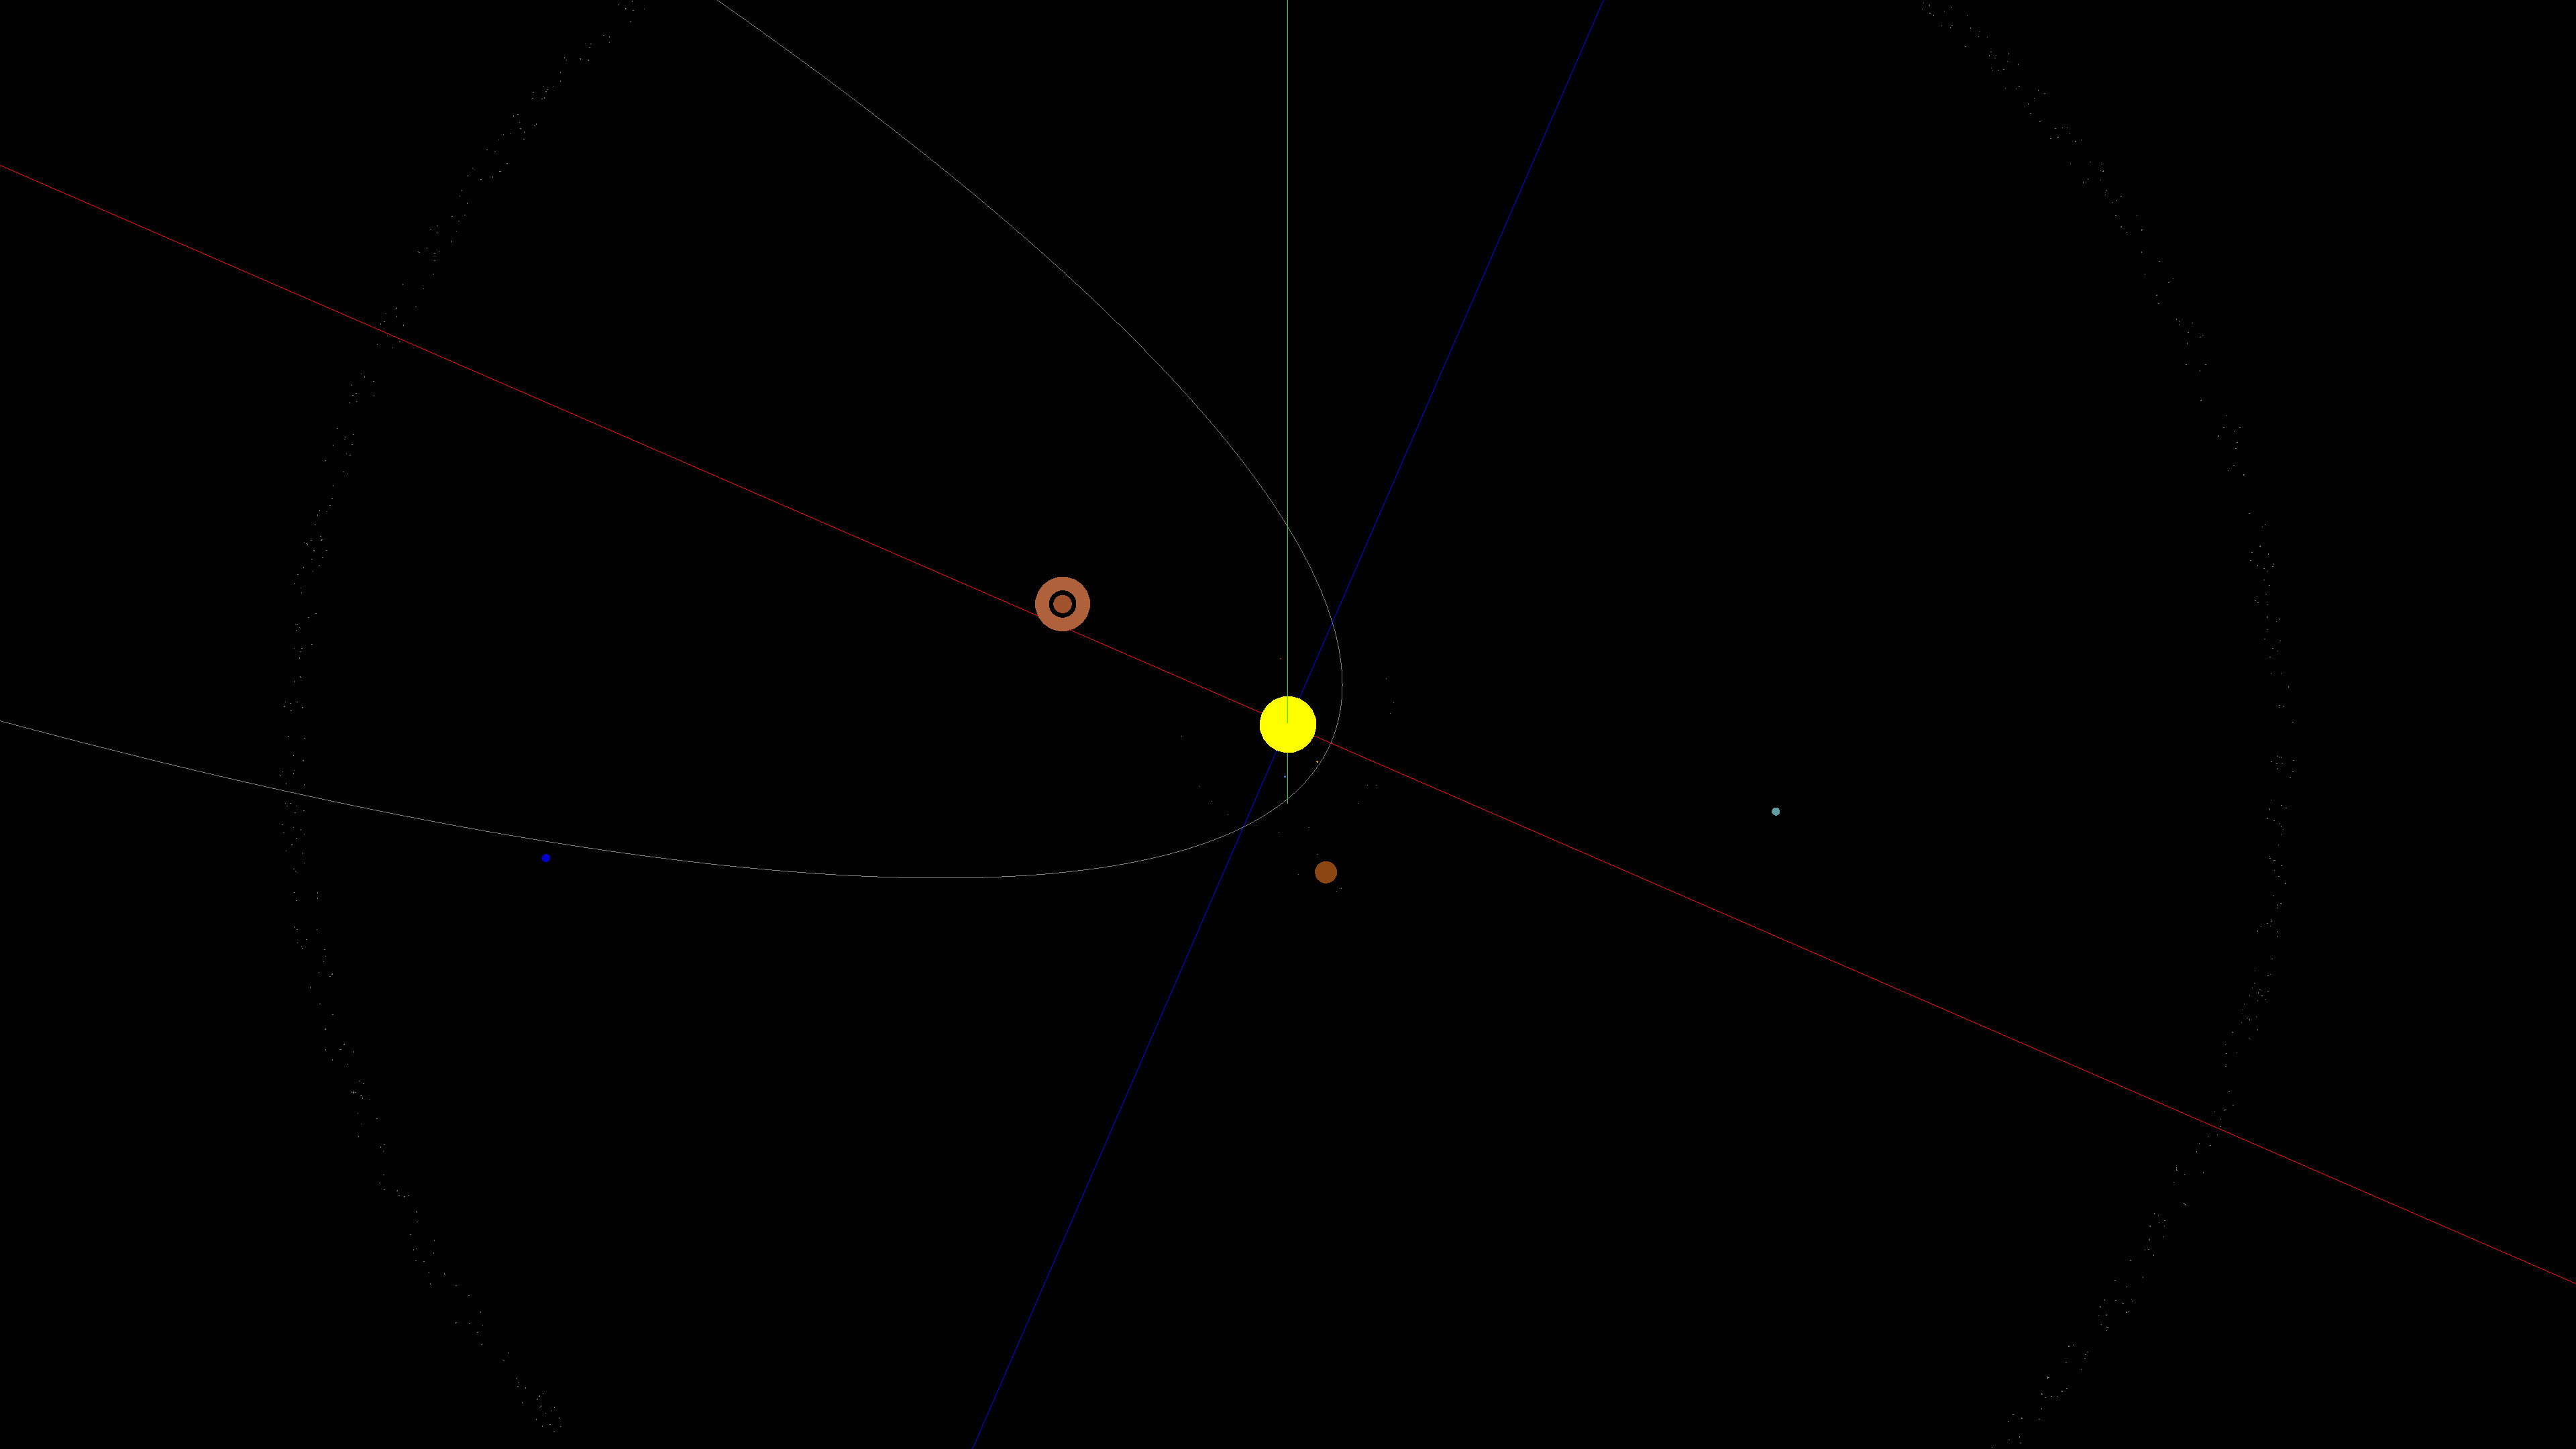
\includegraphics[width=0.7\textwidth]{images/top_view_debug.png}  
    \caption{vista superior do sistema solar em debug mode}
\end{figure}
\begin{figure}[H]
    \centering 
    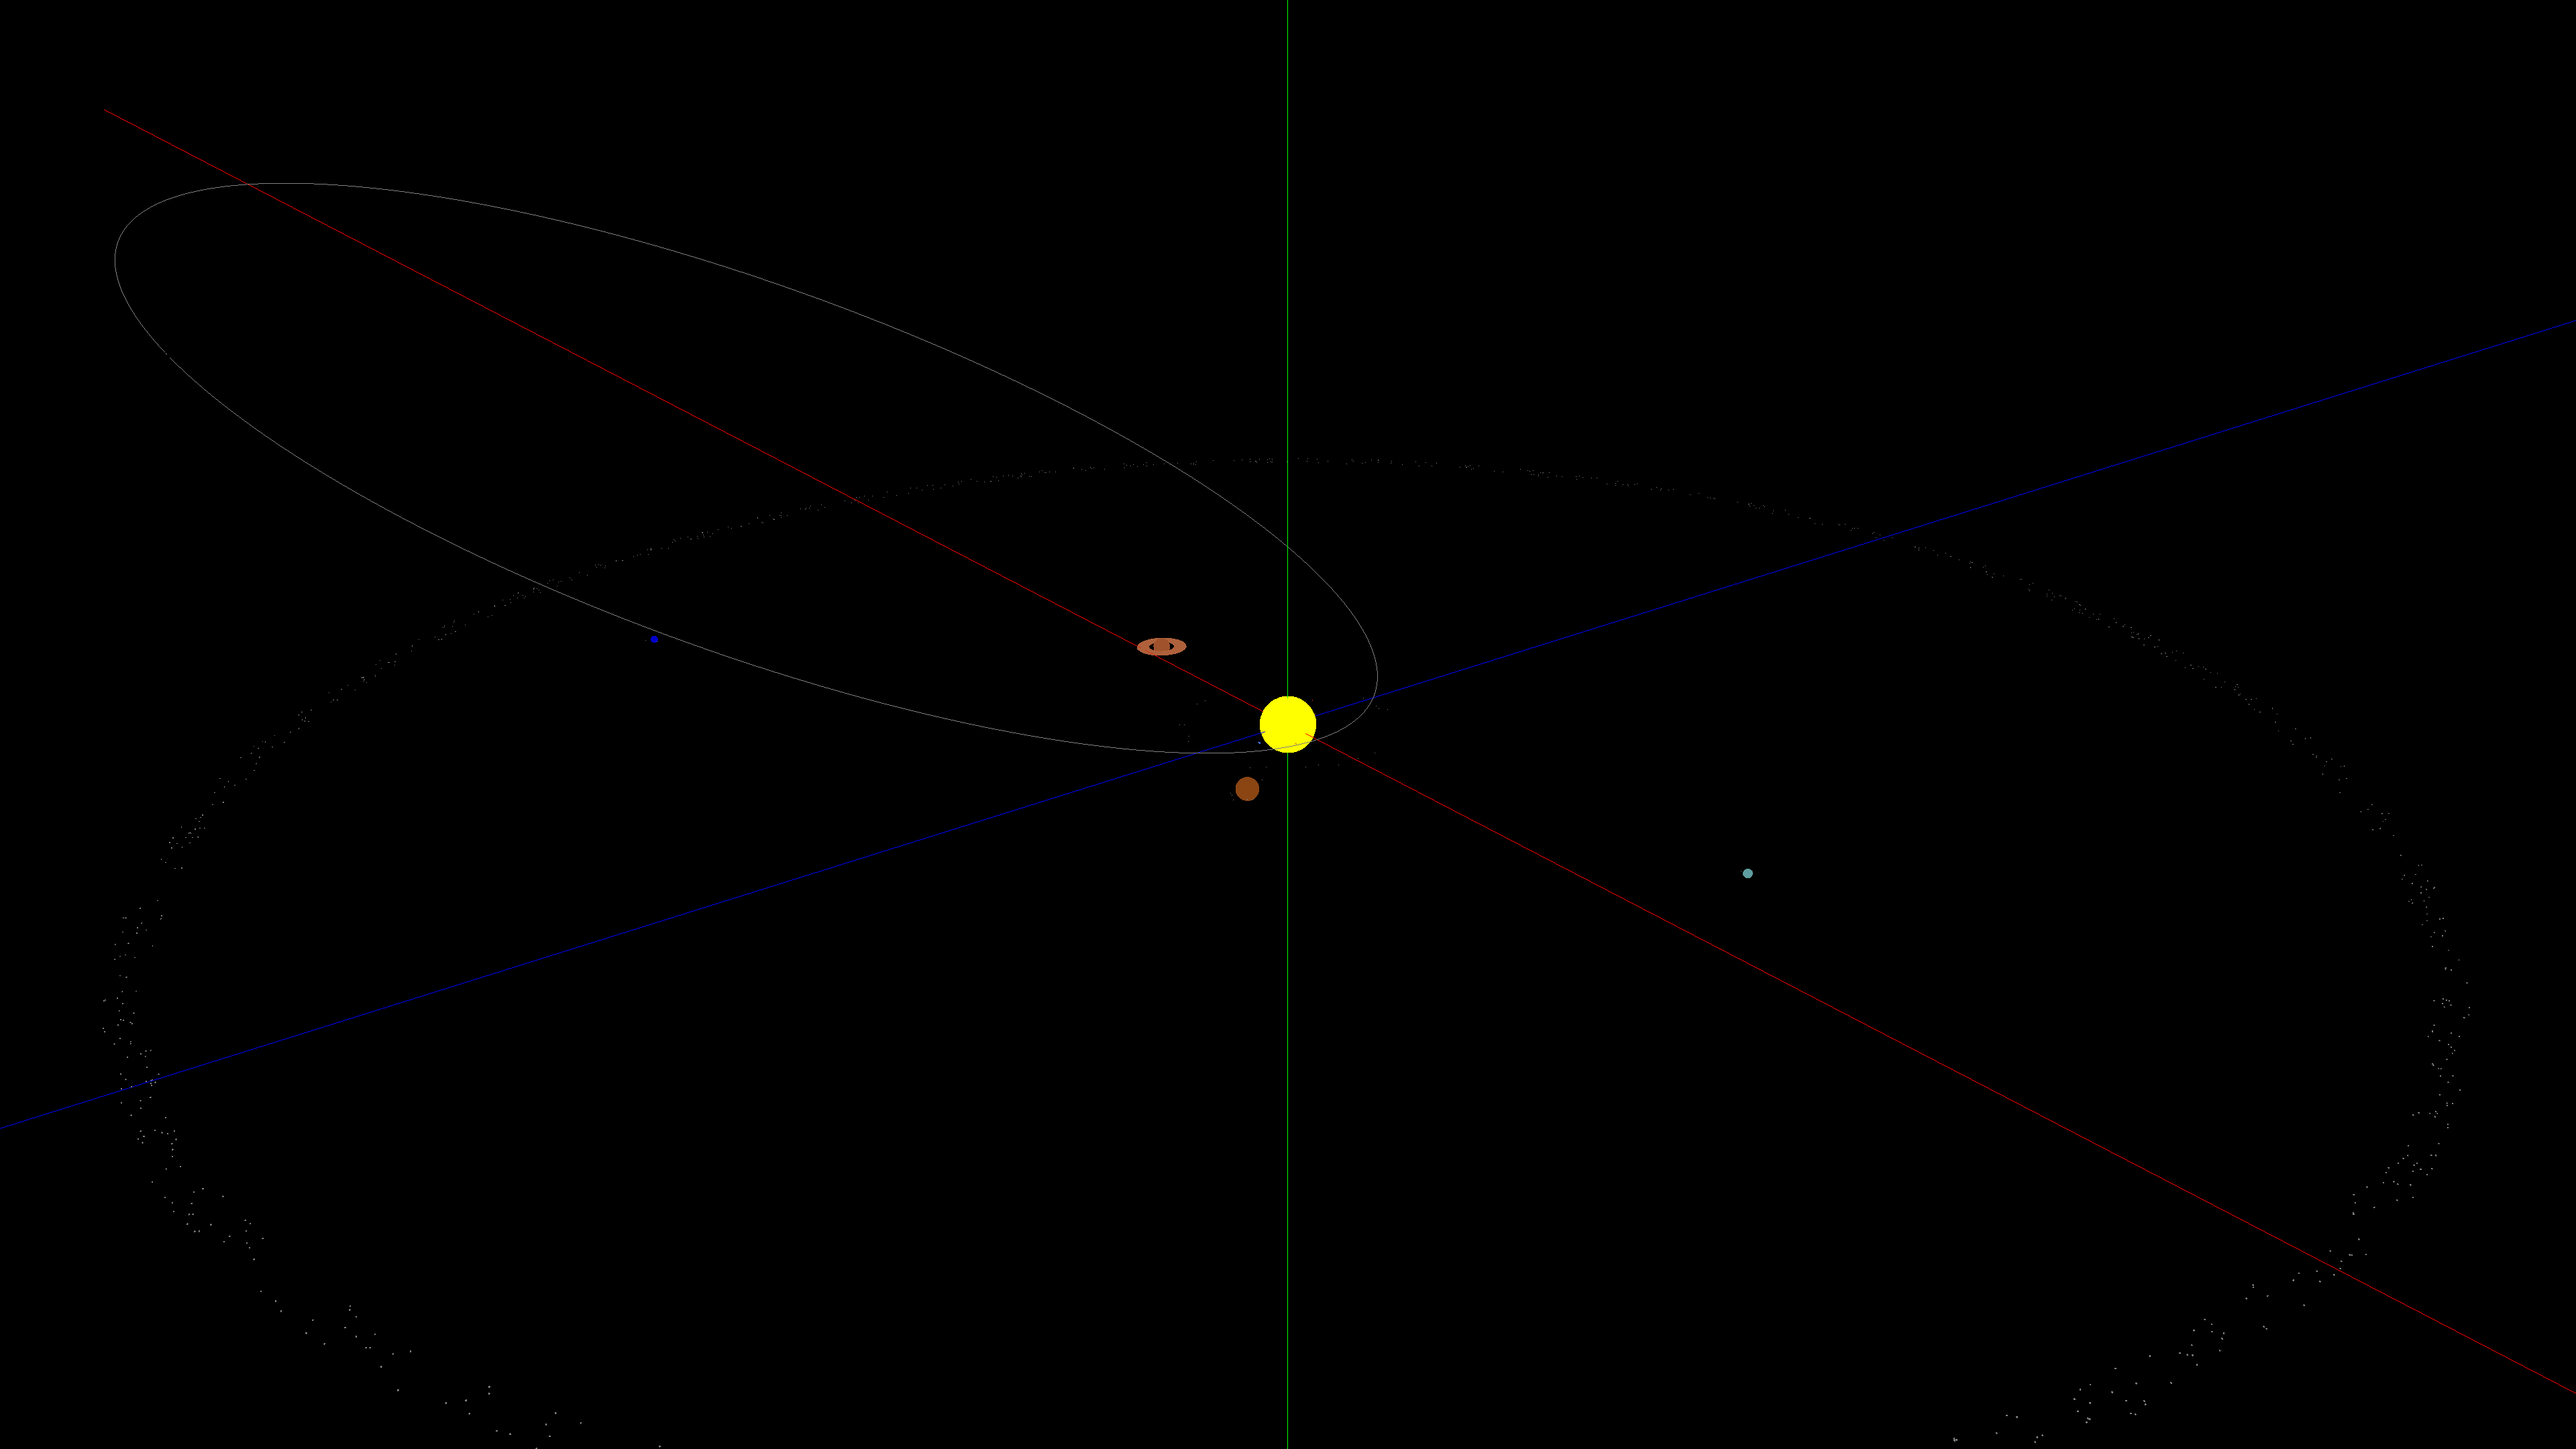
\includegraphics[width=0.7\textwidth]{images/all_view_debug.png}  
    \caption{Vista de toda a órbita do Cometa em cebug mode}
\end{figure}

\chapter{Conclusão}
Com este trabalho prático podemos aplicar os conhecimentos leccionados até agora
nas aulas da unidade curricular de computação gráfica permitindo assim
aprofundar os nossos conhecimentos de openGl.\\
Como trabalho futuro gostaríamos de acrescentar iluminação e texturas, melhorar
as \textit{scenes} criadas até agora para usarem essas melhorias e acrescentar
mais modos à camera.

\end{document}
